\chapter{Сплавленые элементы мощных волокнных лазеров}
\label{ch2}

\section{Сужение оптических волокон (тейпирование)}

Сужение оптического волокна в основном означает его утоньшение. Этот эффект достигается путем нагрева волокна до точки размягчения и последующего вытягивания. Для сужения кварцевых волокон используется тот же самый источник нагрева, что и для сращивания (cваривания).  Ниже операцию сужения оптического волокна будем называть принятым в англоязычной научной литературе термином -- тейпирование (от англ. слова tapering -- сужение). Объект, получаемый после тейпирования, будем называть тейпером (от англ. слова taper -- конус).

\subsection{Распространение излучения через коническое оптоволокно}

Передача излучения по одномодовому волокну происходит благодаря основной (фундаментальной) моде в сердцевине волокна, где число $V$ меньше, чем значение отсечки моды более высокого порядка. При передаче через конус (тейпер), волна встречается с постепенно уменьшающейся сердцевиной и, следовательно, с постепенно уменьшающимся локальным значением $V$ [21]. Это приводит к постепенному изменению распределения поля локальной фундаментальной моды вдоль конуса. Мода распространяется в оболочку с уменьшением $V$. Для любой данной длины волны и профиля показателя преломления оболочки есть диаметр сердцевины, при которой оптический сигнал фактически вырывается из сердцевины и удерживается в промежутке между оболочкой и внешней средой [22, 23]. Эта точка называется точкой перехода конуса. За пределами точки перехода оптоволокно способно поддерживать более одной моды, потому что (а) диаметр оболочки, которая в данном случае образует сердцевину, гораздо больше, чем радиус неконической сердцевины, и (б) различие соответствующих показателей преломления между оболочкой и воздухом очень большое. Эти два эффекта приводят к большому значению $V$, и структура становится многомодовой. Распространение излучения через такую структуру теперь может зависеть от внешних воздействий, которые могут повлиять на затухание поля за пределами волокна.

По мере распространения излучения за пределы минимального поперечного сечения конуса, оно в конце концов встречает конус-вверх, у которого размер сердцевины постепенно увеличивается. Излучение входит в область оболока-воздух, которая по-прежнему способна поддерживать более чем одну моду. Когда сигнал доходит до переходной точки конусности (симметрично расположенной на другой стороне перетяжки), излучение снова начинает удерживаться границей оболочкой с сердцевиной, и, следовательно, мода самого низкого порядка становится единственной распространяющейся модой в неконической области оптоволокна.

Для одномодового конического волокна со ступенчатым профилем, радиус сердцевины $a_0(z)$ уменьшается вдоль оси $z$, и отношение радиуса оболочки $a_1(z)$ к радиусу сердцевины $a_0(z)$ остаётся неизменным.
\begin{equation}\label{eq_ch3_2.18}
  \frac{a_1(z)}{a_0(z)}=\frac{a_1(0)}{a_0(0)}.
\end{equation}
Значение локального $V$ для такой конуса дано как
\begin{equation}\label{eq_ch3_2.19}
  V(z)=V(0)\frac{a_0(z)}{a_0(0)}.
\end{equation}
Если угол достаточно мал, чтобы гарантировать малую связь между фундаментальной модой и модами более высокого порядка, говорят, что конус адиабатический. В этом случае вся энергия сохраняется в основной моде. Если угол конусности недостаточно мал, потеря связанной энергии становится существенной, и конус становится не адиабатическим или с потерями.

Бесконечно большой адиабатический конус с параболическим профилем показателя преломления определяется на расстоянии $z$ от входа как
\begin{equation}\label{eq_ch3_2.20}
  n^2(R)=n_0^2(1-2\Delta R^2),
\end{equation}
где $R=r/a_0$ есть нормированное радиальное расстояние. Размер локальной точки (спота) $\omega(z)$ нормированный на начальный радиус $a_0(0)$ дается как
\begin{equation}\label{eq_ch3_2.21}
  \frac{\omega(z)}{a_0(0)}=\frac{\omega(0)}{a_0(0)}\sqrt{\frac{V(z)}{V(0)}}.
\end{equation}
Он линейно увеличивается с увеличением $a(z)$ или уменьшением соотношения конусности. В случае неадиабатического конуса размер пятна определяется суммарным полем. Оно является результатом суперпозиции модовых полей в поперечном сечении области сердцевина-оболочка, фундаментальной моды и оболочечных мод более высокого порядка. В случае конечного размера оболочки неадиабатического конуса со ступенчатым профилем показателя преломления с линейной формой конуса, мы имеем
\begin{equation}\label{eq_ch3_2.22}
  a_0(z)=a_0(0)[1-(z/L)],
\end{equation}
где $L$ является длиной конуса.

Рассмотрим одномодовое волокно, чья основная мода находится в возбужденном состоянии. Мощность основной моды любой неоднородностью, нарушающей цилиндрическую симметрию, связывается с полем излучения (radiation field). В случае оптоволокна с конечной оболочкой мощность теряется за счет связи между основной модой и модами оболочки. Длина связи $L_C$ определяется константами распространения $\beta_1$ основной моды и $\beta_2$ мод оболочки:
\begin{equation}\label{eq_ch3_2.23}
  L_C=2\pi/(\beta_1-\beta_2).
\end{equation}
В случае тейпера масштаб длины $L'$ определяется через угол $\Omega(z)$ между касательной к границе сердцевина-оболочка и осью оптоволокна. Если $a(z)$ -- локальный радиус, мы имеем
\begin{equation}\label{eq_ch3_2.24}
  \tan\Omega(z)=a(z)/L',
\end{equation}
где $L'$ является расстоянием вдоль оси конуса от апекса до конуса, образованного половиной угла $\Omega(z)$. Если величина длины $L'$ неоднородности больше, чем длина волны электромагнитного поля, наблюдаются затухание или рассеяние, потому что при таком масштабе длин поле становится чувствительным к неоднородностям. Если  $n_1 \approx n_2 \approx n$ (приближение слабого волновода), потери существенны, когда $\lambda/n < L'$. Значительные потери возникают, если величина длины неоднородности (конусности) ограничена примерно
\begin{equation}\label{eq_ch3_2.25}
  \frac{\lambda}{n} < L' < L_C.
\end{equation}
Таким образом, для адиабатического конуса $\tan\Omega(z) \approx \Omega(z)$ и уравнение \eqref{eq_ch3_2.23} указывает на то, что, если $L'>L_C$, мы имеем малые или эквивалентные потери, если
\begin{equation}\label{eq_ch3_2.26}
  \Omega(z)<a(\beta_1-\beta_2)/2\pi.
\end{equation}
Угол конусности должен быть достаточно мал и удовлетворять уравнению \eqref{eq_ch3_2.26} в каждой точке вдоль конуса. Для достаточно медленной конусности фронт волны остаются почти практически плоскими. При значительной конусности (gradual taper), которая может поддерживать многомодовое распространение излучения в увеличенной части конуса, преобразование основной моды в моды более высокого порядка или моды излучения должно быть пренебрежимо малы.

\subsection{Тейпирование одномодовых оптических волокон}
%\label{ssub:subsubsection_name}

Тейпирование одномодового волокна должно осуществляться достаточно медленно. Если тейпирование будет резким, то оптическая мощность фундаментальной моды перейдет к модам более высокого порядка (МВП). Обычно это приведет к высоким потерям в тейпере. Пока изменение радиуса сердцевины волокна ($\Delta r$) мало относительно длины биений ($L_B$) между фундаментальной модой и первой МВП, тейпер является медленно изменяющимся («медленный» тейпер) [60-63]. Это формулируется следующим образом:

\begin{equation}\label{eq2.14}
  \frac{\Delta r}{r} \ll 1.
\end{equation}
где $r$ -- радиус сердцевины волокна. Локальное изменение радиуса сердцевины волокна в зависимости от длины биений может быть записано как $\Delta r=L_B (dr/dz)$,  где $dr/dz$ -- локальный наклон тейпера. Длина биений между основной модой и МВП может быть выражена как

\begin{equation}\label{eq2.15}
  L_B=\frac{2\pi}{\beta_1-\beta_2},
\end{equation}
где $\beta_1$ и $\beta_2$ -- коэффициенты распространения фундаментальной моды (распространяющейся по сердцевине волокна) и МВП, соответственно. Подставляя выражение для локального наклона тейпера в уравнение \eqref{eq2.14} можно найти критерий, который должен быть выполнен для тейпера с низкими потерями. Его называют \textit{адиабатическим критерием}.

\begin{equation}\label{eq2.16}
  \frac{dr}{dz}\le\frac{r}{L_B}=\frac{r}{2\pi}(\beta_1-\beta_2)
\end{equation}
В адиабатическом критерии $\beta_2$ относится к коэффициенту распространения первой МВП. Эта мода будет иметь самый близкий к основной моде коэффициент распространения, и даст самое большое значение длины биений. Это означает, что самый строгий критерий устанавливается при использовании в расчете именно этой моды.

Для линейного профиля тейпера наклон тейпера ($dr/dz$) будет одинаковым по всей длине тейпера. Таким образом, максимальная длина биений ($L_{B, max}$) и полное отношение тейпера ($TR$) определяют длину адиабатического тейпера ($L$). Соотношение тейпера определяется как $TR = r_1/r_2$, где $r_1$ и $r_2$ -- радиусы сердцевины волокна на нетейпированном и тейпированном концах волокна,
соответственно. Уравнение \eqref{eq2.16} может быть приведен к (см. приложение 1),

\begin{equation}\label{eq2.17}
  L \ge (TR-1)L_{B, max}.
\end{equation}

Для адиабатического тейпера излучение в фундаментальной моде оптического волокна останется без изменений (без переизлучения в МВП). На рис.~\ref{img:taper_review_2_8} показан расчетный MFD фундаментальной моды тейпированного волокна со ступенчаты профилем ПП (a) и в PCF (b). Оба расчета сделаны на длине волны 1064 нм программой MIT Photonics Band [??]. Волокно со ступенчатым профилем ПП имеет постоянный NA=0,14 и становится ММ при диаметре сердцевины свыше 5,7 мкм. MFD волокна со ступенчатым профилем ПП следует за диаметром сердцевины пока V-параметр не достигает единицы. Далее мода быстро расширяется. Это хорошо согласуется с аналитическим выражением для MFD волокна со ступенчатым профилем ПП, показанного на рис.~\ref{img:taper_review_2_2}.

\begin{figure} [ht]
  \center
  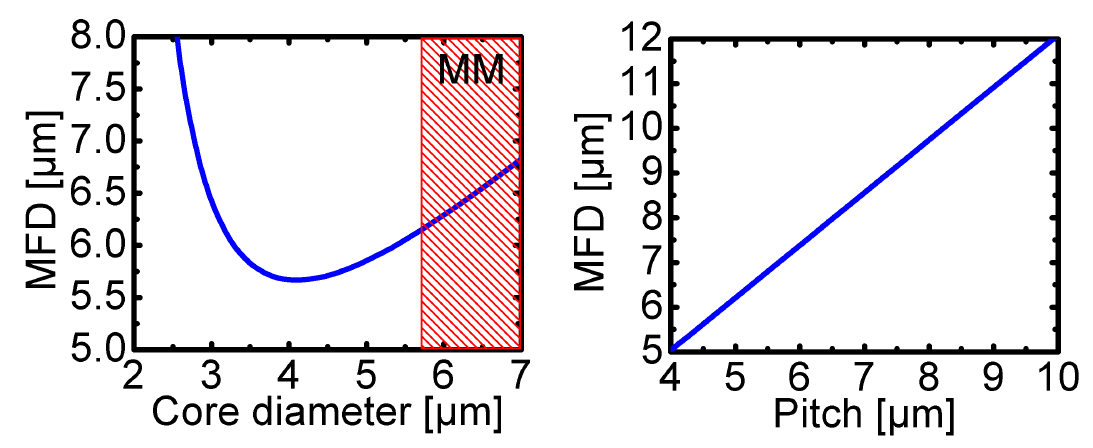
\includegraphics [scale=0.4] {taper_review_2_8}
  \caption{(a) MFD тейпированного волокна со ступенчатым профилем ПП. (b) MFD тейпированного PCF.}
  \label{img:taper_review_2_8}
\end{figure}

\begin{figure} [ht]
  \center
  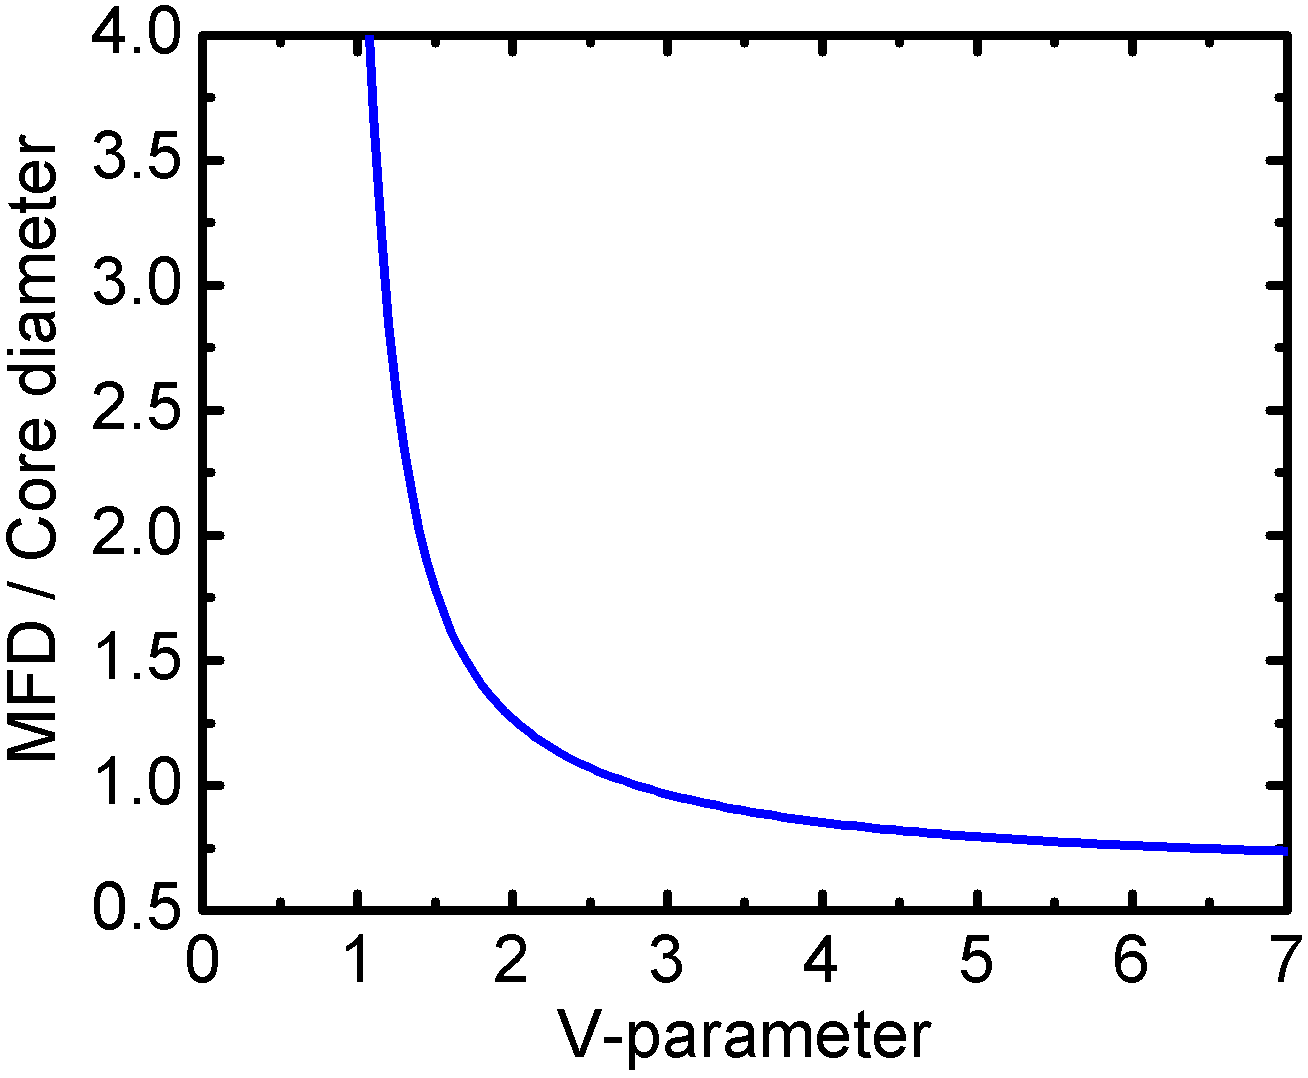
\includegraphics [scale=0.2] {taper_review_2_2}
  \caption{Нормированный MFD как функция V-параметра для фундаментальной моды в волокне со ступенчатым профилем ПП.}
  \label{img:taper_review_2_2}
\end{figure}

\subsection{Тейпирование многомодовых оптических волокон}

У тейперов из ММ волокна обычно возбуждается много мод, поэтому адиабатический критерии из уравнения \eqref{eq2.16} уже не может использоваться. Вместо этого изменение радиуса сердцевины ММ волокна ($\Delta r$) более чем на половину периода луча ($z_p$) должно быть малым [60]. Половина периода луча показана на рис.~\ref{img:taper_review_2_9}. Тогда получим адиабатический критерии, подобный критерию для тейперов из одномодового волокна, но с длиной биений, замененной на половину периода луча

\begin{equation}\label{eq2.18}
  \frac{dr}{dz}\le\frac{r}{z_p}.
\end{equation}

Для заданного NA у луча, который проходит через ось оптического волокна (меридиональный луч), будет самая длинная половина периода луча. Для такого луча половина периода определяется как

\begin{equation}\label{eq2.19}
  z_p=\frac{2r}{\tg\theta_z}.
\end{equation}

Вставляя выражение для $z_p$ в адиабатические критерии, получим

\begin{equation}\label{eq2.20}
  \frac{dr}{dz}\le\tg\theta_z/2.
\end{equation}

\begin{figure} [ht]
  \center
  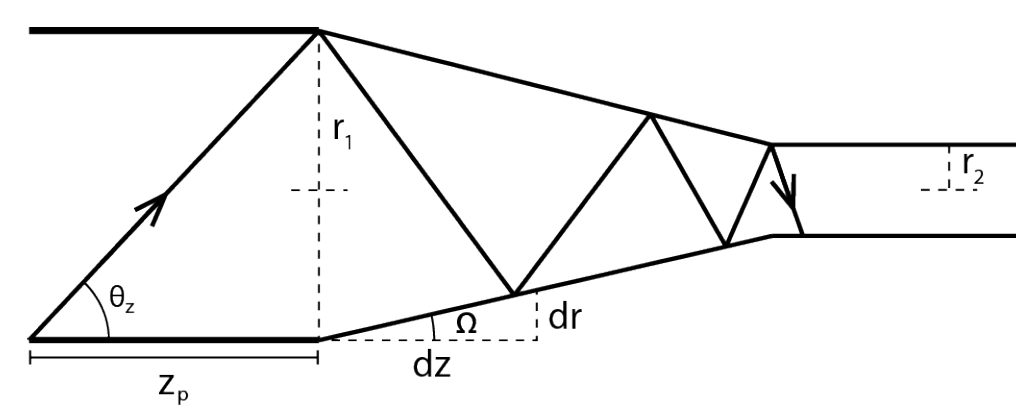
\includegraphics [scale=0.4] {taper_review_2_9}
  \caption{Тейпирование ММ волокна.}
  \label{img:taper_review_2_9}
\end{figure}

Фактор $dr/dz$ также может быть описан как локальный угол ($\Omega$)
(см. рис.~\ref{img:taper_review_2_9}). Адиабатический тейпер обеспечивается, если угол луча в два раза больше угла тейпера в любой точке вдоль тейпера ($2\Omega \le \theta_z$).

Для линейного профиля тейпера может быть выведена минимальная длина тейпера для ММ волокна, которая гарантирует выполнение адиабатического критерия. Так же, как и для тейпера из SM волокна, минимальная длина тейпера (см. приложение 2),

\begin{equation}\label{eq2.21}
  L \ge \frac{D_1-D_2}{\tg\theta_z}.
\end{equation}

Минимальная длина тейпера из линейно тейпированного ММ волокна будет зависеть от NA введенного в волокно излучения. Например, для введенного излучения с NA=0,22, и с показателем преломления сердцевины волокна $n_{co} = $1,45, угол для меридионального луча равен $\theta_z=\sin^{-1}(NA/n_{co})=$8,7. С данным NA и для ММ волокна тейпированного с линейным профилем из диаметра $D_1 =400$ мкм в $D_2 =150$ мкм, минимальная длина тейпера будет составлять $L_{min} = $1,6 мм.

Для тейпированного волокна с двойной оболочкой адиабатический критерий должен быть выполнен как для сигнальной сердцевины, так и оболочки накачки. При большой площади моды (LMA) сигнальной сердцевины адиабатический критерии для сердцевины обычно будут самыми строгими и поэтому будут определять минимальную длину тейпера.

Для пассивных оптических устройств яркость сохраняется (теорема яркости) [65]. Яркость излучения $L_R$ определяется как мощность на площадь на телесный угол ($W/m^2/sr$)

\begin{equation}\label{eq2.22}
  L_R=\frac{\Phi}{A\Omega},
\end{equation}
где $\Phi$ -- поток через данную площадь $A$, а $\Omega$ есть телесный угол. Первоначально яркость определялась как яркость излучающего предмета, воспринимаемая человеческим глазом [66]. Однако термин стал стандартным в применении к лазерам и поэтому будет использован далее в тексте.

Из теоремы яркости следует, что адиабатически тейпированное ММ волокно сохраняет яркость. Для ММ волокна $A = \pi r^2$, где $r$ есть радиус сердцевины
волокна. Телесный угол $\Omega = 4\pi\sin^2(\theta/2)$, где $\theta$ -- полуугол расходимости. Поток равен мощности $P$ проходящей через волокно. Поэтому яркость излучения в ММ волокне ($L_{MM}$) может быть записана как

\begin{equation}\label{eq2.23}
  L_{MM}=\frac{P}{\pi r^2\pi\sin^2\theta}.
\end{equation}
Для адиабатического тейпера без потерь сохранение яркости означает, что соотношение между NA и диаметром сердцевины $D$ в конце и начале тейпера может быть выведено как

\begin{equation}\label{eq2.24}
  D_{in}\sin\theta_{in}=D_{out}\sin\theta_{out} \Rightarrow D_{in}NA_{in}=D_{out}NA_{out},
\end{equation}
где $D$ -- диаметр сердцевины ММ волокна, NA -- числовая апертура излучения. Уравнение показывает, что для адиабатического сохраняющего яркость тейпера из ММ волокна диаметр сердцевины умноженный на NA излучения является константой.

\newpage
\section{Изготовление сплавленых объединителей накачки высокой мощности}
%\label{sec:section_name}

\subsection{Последовательность и параметры управления технологическим процессом}

\begin{figure} [ht]
  \center
  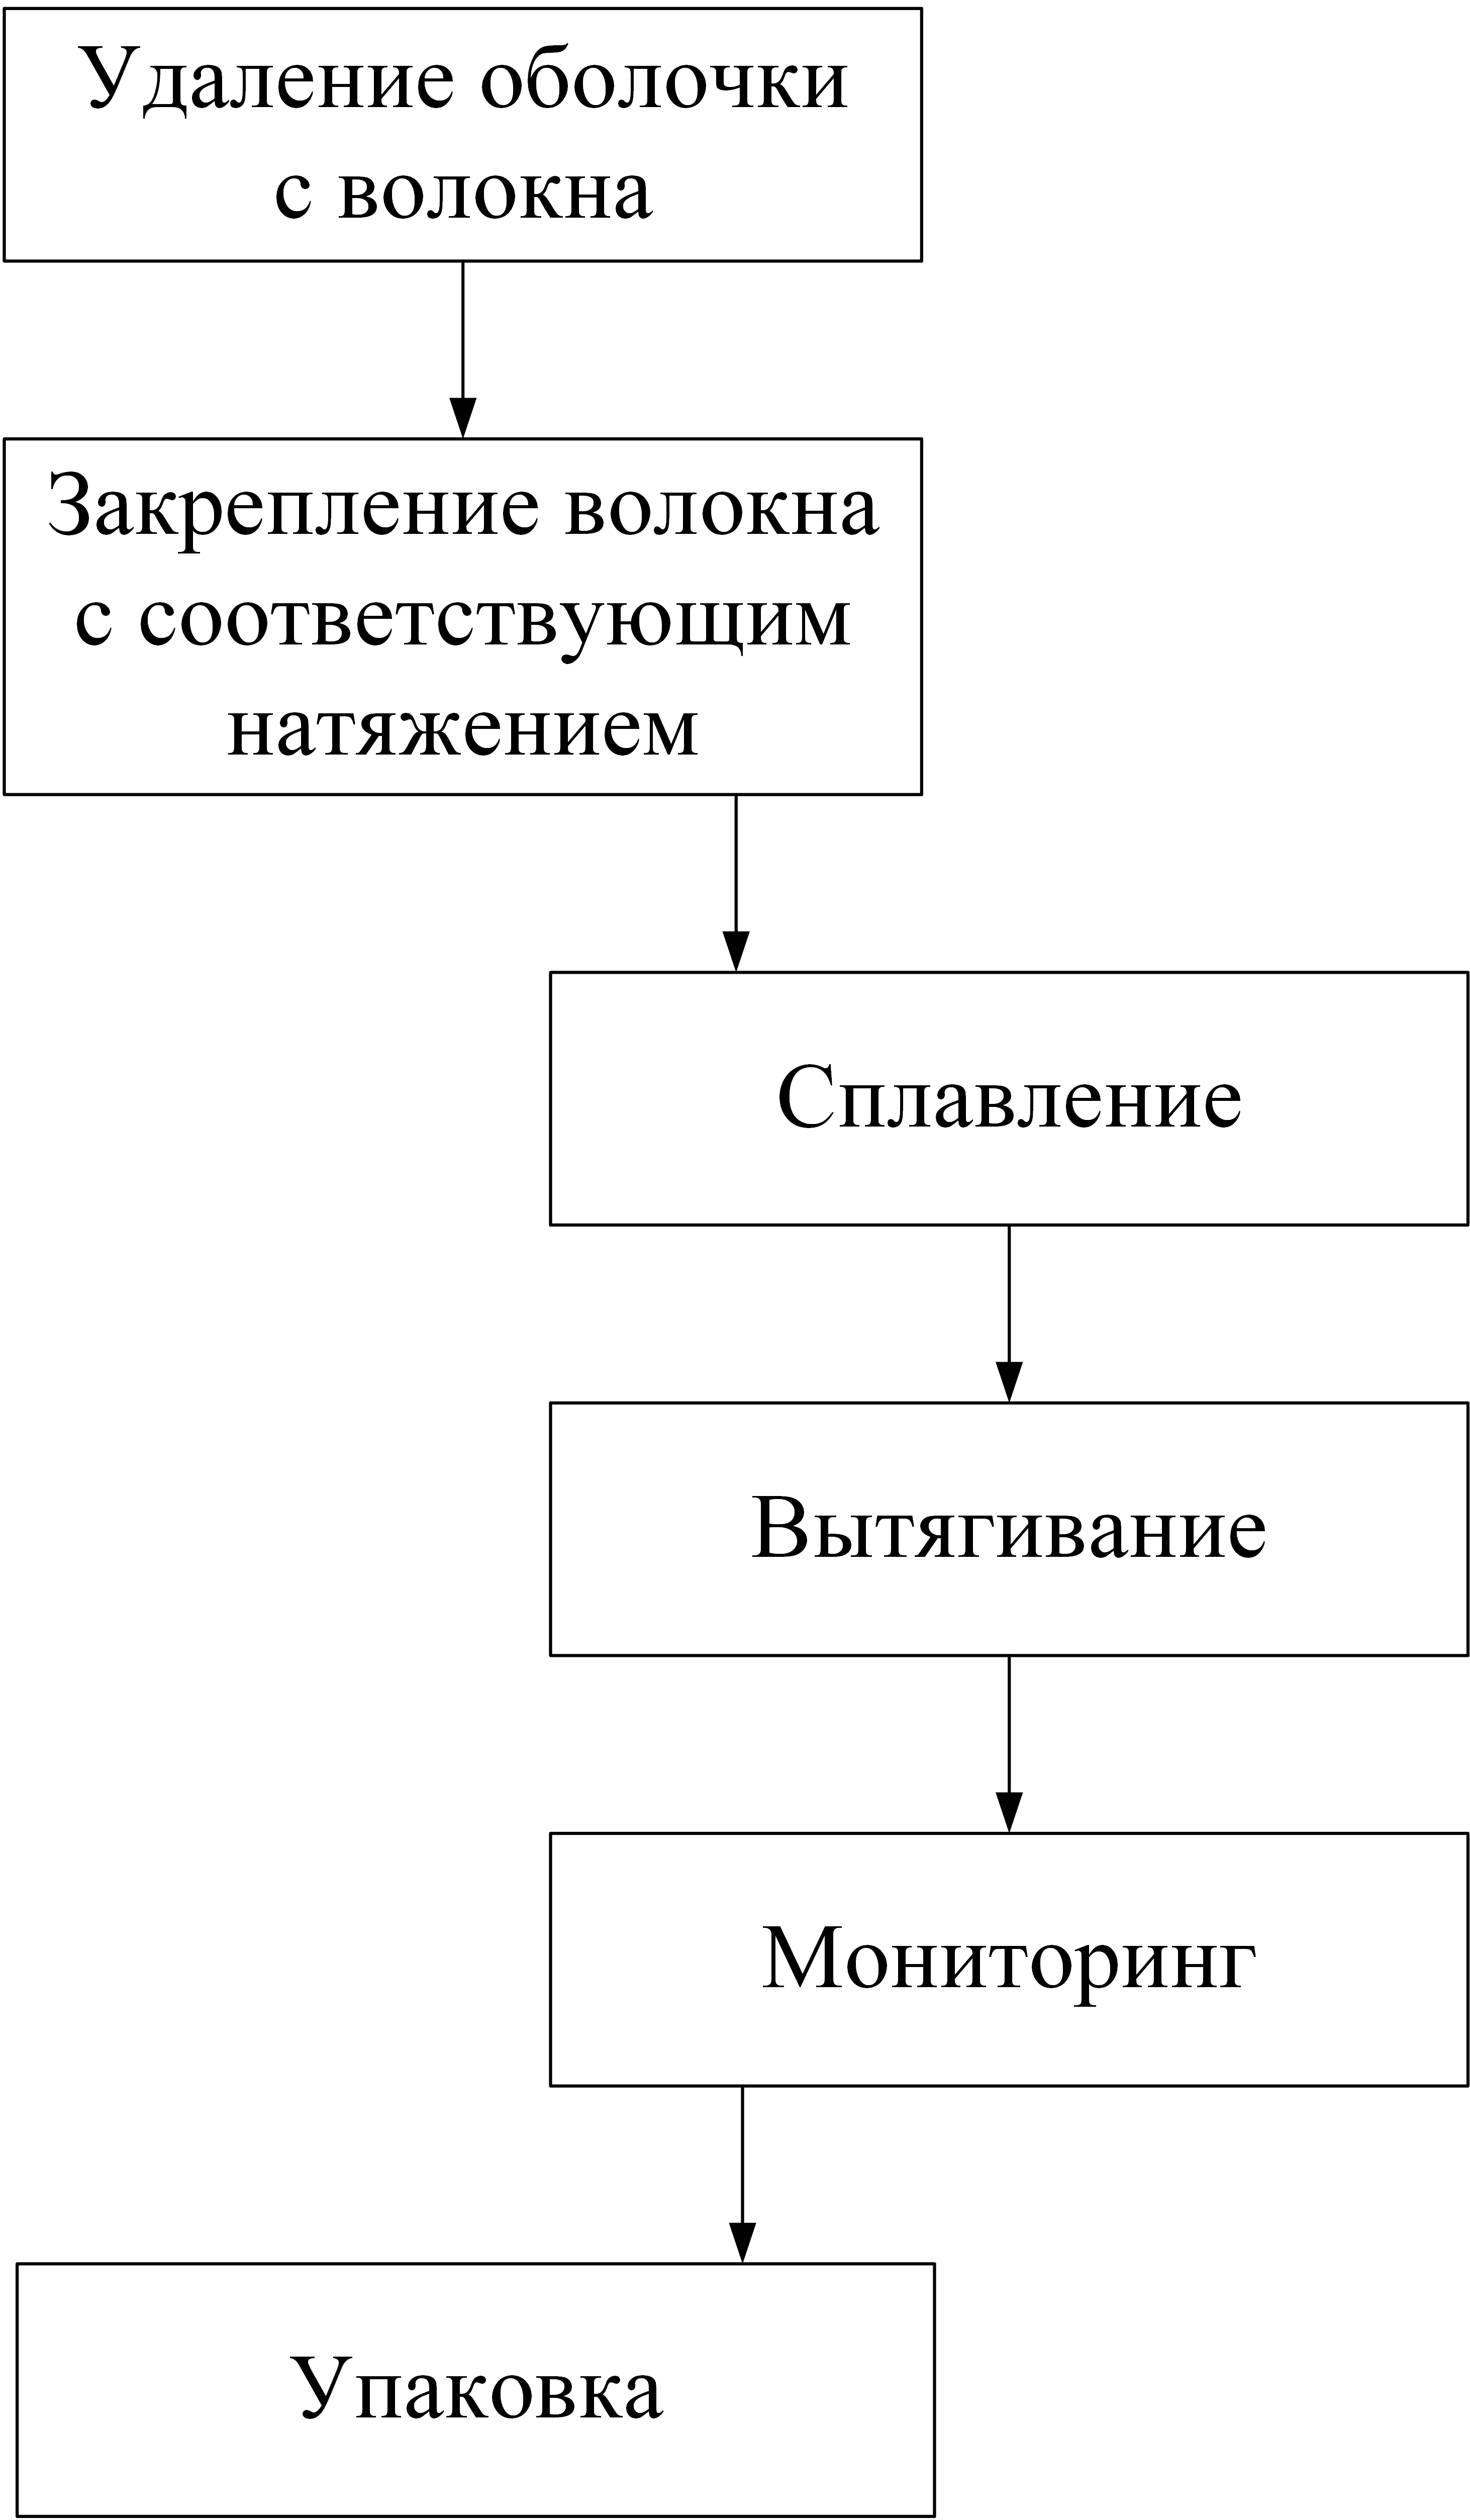
\includegraphics [scale=0.4] {taper_review_ch3_2_7}
  \caption{Процесс изготовления оптоволоконных каплеров.}
  \label{img:taper_review_ch3_2_7}
\end{figure}

Процесс изготовления каплеров из оптоволокна показан на рис.~\ref{img:taper_review_ch3_2_7}. Он включает в себя снятие защитного покрытия оптоволокна, установку оптоволокна, расплавление, вытягивание, мониторинг связи и упаковку. Ниже даные этапы описаны подробнее.

\begin{enumerate}

\item{\textbf{Снятие защитного покрытия оптоволокна}}

С оптоволокна, по которому будет проходить сигнал, и еще один кусок оптоволокна небольшой длины (приблизительно 2 метра) очищается от защитного акрилатного покрытия с помощью стриппера на длине порядка 25 мм. Затем они располагаются параллельно друг другу на поверхности оптического стола. Полученные зачищенные участки оптоволокна проходят тщательную очистку с помощью спирта или специального очищающего раствора. Это важный шаг, поскольку любая микроскопическая примесь (пыль или частицы пластика), оставшаяся на поверхности волокна, может привести к потерям на рассеяние и снизить общую производительность устройства.

По той же причине обычно изготовление каплеров выполняется в относительно чистой среде. В нашем случае это чистое помещение класса ISO5. Кроме того, в ходе очистки оптоволокна от защитной оболочки более предпочтительно использование пластиковых стрипперов, поскольку их применение не приводит к появлению в волокнах микротрещин.

\item{\textbf{Расположение оптоволокна на держателях (зажимах)}}

Далее пара волокон скручивается, чтобы обеспечить плотный контакт в продольном направлении вдоль зачищенного участка, и зажимаются на противоположных концах трансляционной подвижки с помощью специально созданных в размер оптоволоконных зажимов. Скрутка волокон должна быть локальной (только в зачищенной зоне) и симметричной относительно центра зачищенного участка.

\item{\textbf{Расплавление и вытягивание}}

Как только оптоволокно размещено соответствующим образом, два выходных волоконных канала присоединяются к блоку фотодетекторов, и включается излучение лазерного диода на входе. Затем автоматизированная система в реальном времени на дисплее ПК отображает величину потерь и связанную мощность. На данном этапе соответствующим образом может быть отрегулирован уровень максимальной мощности входного сигнала. Это значение записывается системой как уровень входной мощности и используется для расчёта потерь мощности излучения формируемого волоконно-оптического устройства.

Когда во входном канале фиксируется подходящий уровень мощности, запускается непосредственно сам процесс изготовления. Все двигатели последовательно активируются, и горелка располагается внизу под зачищенным участком пары скрученных волокон. Для того, чтобы избежать провисания размягченного оптоволоконного материала, что может привести к большим потерям в работе каплера, к оптоволокну посредством медленного вытягивание прикладывается небольшое натяжение. Можно утверждать, что, если в ходе вытягивания каплера зафиксировано провисание волокон, это означает, что оператор не контроллирует технологический процесс и соответственно его результат.

Расплавление и вытягивание приводят к возникновению связи (передачи) мощностей, вначале с малой скоростью, а в конце с всевозрастающей скоростью обмена мощностями между волокнами. Это хорошо видно на монитора ПК, на котором изображен онлайн-график измеренной мощности в обоих выходных каналах в зависимости от степени удлинения. Взаимодействие начинается обычно через 6-7 минут с начала вытягивания. В этот момент времени программа на ПК запускает автоматическую запись данных, относящихся к взаимодействию мощностей. Программа постоянно сравнивает мгновенные измеренные значения с предварительно запрограммированными параметрами. Когда эти два набора данных становятся идентичными или практически идентичными, программа управления инициирует сигнал на удаление горелки из-под пары оптоволокон, при этом отключаются двигатели подвижки. Как только заканчивается изготовление каплера начинается контроллируемый процесс упаковки. Во ходе процесса упаковки монитор отображает мгновенный коэффициент разделения (splitting ratio), уровень потерь (excess loss), вносимые потери (insertion loss) и абсолютные  мощности в пропускающем и связанном каналах.

\item{\textbf{Упаковка}}

Упаковка созданных FBT-каплеров – важный шаг, поскольку устройство очень хрупкое и может быть легко повреждено. Применяемый метод полной упаковки каплера занимает 10-15 минут.

\end{enumerate}

%\subsection{Параметры управления}

Для того, чтобы достичь целевых технических харатеристик, процесс изготовление FBT-каплера требует пристального контроля [31]. Ниже описаны основные параметры управления изготовлением FBT-каплеров. Коэффициент спектрального разделения в каплере является функцией коэффициента связи, который зависит от длины волны и варьирующийся от точки к точке вдоль каплера, максимален в перетяжке и снижается при движении к краям биконического тейпера [17]. Точная величина коэффициента связи определяется геометрией каплера и формой конуса. Профиль продольного конуса и размер перетяжки фактически задают форму конуса, что в конечном итоге определяет производительность каплер при данной длине волны. Эти два параметра могут быть заданы путем изменения скорости вытяжки, длины зоны нагрева и тепературы нагревателя (горелки). По существу, игра этими переменными можно получить различные формы конусов, что подразумевает вариации растояния между сердцевинами волокон, профиля перетяжки, наклона конуса и длины связи (взаимодействия). Конический переход преобразует локальную фундаментальную моду распространяющейся по серцевине неконического оптоволокна в оболочечную моду в зоне перетяжки конуса. Для достижения малого уровня потерь из-за преобразования в моды более высокого порядка требуется, чтобы конический переход был адиабатическим [32, 33].

\textbf{Регулировка температуры:} Параметры источника нагрева (нагревателя) оказывает значительное влияние на физическую форму конуса а, следовательно, и на его характеристики. Нагреватель должен обеспечивать воспроизводимый (повторяемый) профиль температуры, которым можно управлять посредством регулировки скорости газового потока. Длина и форма пламени являются самыми важным фактором управления профилем конуса. Волоконные компоненты, сделанные на основе одномодовых оптоволоконных тейперов, обладают уникальные проводящими характеристиками, определяемыми формой конуса. На практике конус любой формы может быть образован соответствующим управлением температурным профилем нагревателя, длиной зоны нагрева и нагрузкой, приложенной к оптоволоконному жгуту во ходе расплавления.

\textbf{Ширина зоны нагрева:} Продольный профиль конуса обычно определяется длиной зоны нагрева во время процесса вытяжки. Длина нагретой части оптоволокна может быть разной и изменяться посредством изменения уровня пламени во время огневой полировки. При огневой полировке перемешающееся пламя в определённое время нагревает заданный участок оптоволокна. Горелка устроена таким образом, чтобы двигаться вдоль оптоволокна с определённой скоростью в обоих направлениях. Во время каждого цикла передвижения пламя греет каждый бесконечно малый элемент вдоль оптоволокна [34]. Если нагреваемый отрезок оптоволокна остаётся неизменным по времени, результирующий профиль конуса принимает экспоненциальную форму. Состояние фиксированной длины зоны нагрева достигается применением либо стационарного пламени, либо движущейся горелкой, имеющей постоянную длину зоны нагрева (ширину пламени).

Таким образом, когда оптоволокно вытягиваются, его диаметры в зоне нагрева уменьшаютс и материал перераспределяется в виде конуса. Поскольку длина зоны остается постоянной, объём размягчённого кварца из-за тейпирования сокращается. Это приводит к получению экспоненциальной формы конуса [23]
\begin{equation}\label{eq_ch3_2.27}
  r(z)=r_0 e^{z/\Delta z},
\end{equation}
где $r(z)$ является радиусом конического поперечного сечения при любом $z, \Delta z$ есть ширина пламени, и $r_0$ -- радиус перетяжки. Если $h$ -- ширина пламени, то длина зоны нагрева составляет $h+\Delta z$. Таким образом, при помощи изменения ширины пламени становится возможным изменение длины перетяжки конуса.

\textbf{Скорость вытягивания:} Температурой расплавления можно управлять посредством изменения температуры пламени и скорости вытягивания оптоволокна. Скорость вытягивания регулируется путем изменения приводной мощности двигателей, передвигающих подвижки. Нужно добиться минимального натяжения при расплавлении, но при этом достаточного, чтобы избежать любого провисания размягченных волокон. Манипулированием температурой нагрева волокон, изменением их расположения отностиельно пламени, временем нагрева и скоростью вытягивания можно достич практически любой степени расплавления. Степень расплавления вместе с длиной вытягивания задают форму поперечного сечения тейпера.

Сила связи имеет сильную функциональную зависимость от межцентрового разделения между волокнами и окончательного размера перетяжки тейпера в поперечном сечении. Степень сплавления $f$ описывется аналитическим выражением, которое с достаточной степенью точности дает количественную оценку этим двум параметра посредством соотношения [35]
\begin{equation}\label{eq_ch3_2.28_1}
  d=2b(1-f(2-\sqrt{2})),
\end{equation}
где $2b$ есть диаметр нетейпированного оптоволокна. Степень сплавления $f$, ктороая удовлетворяет соотношению $0 \le f \le 1$, где $f=0$ соответствует случаю <<изолированного>> оптоволокна и $f=1$ относится к форме, при которой два оптоволокна были полностью сплавлены до образования круглого поперечного сечения.

Для заданного уровня сплавления и продольного профиля, может быть достигнут любой необходимый размер поперечного сечения каплера в перетяжке путем регулировки длины вытяжки. На практике поперечное сечение перетяжки управляется посредством манипулирования профилем конуса с помощью варьирования ширины пламени. Для одной и той же длины вытяжки большая ширина пламени о даёт более широкое поперечное сечение перетяжки. Малый размер поперечного сечения перетяжки при малом размере каплера приводит к формированию крутого (с большим углом) конуса и относительно большим потерям [17]. В управляемой посредством ПК системе изготовления длина вытяжки всегда определяется заранее через заданное программно соотношение разделения (splitting ratio). Однако, для фиксированного размера перетяжки каплера для разных степеней сплавления или различной ширины пламени длина вытяжки может быть различной. Иными словами, все указанные параметры являются связанными.

 \subsection{Изготовление сплавленых объединителей накачки на волокне с двойной оболочкой}

Накачка и сигнальное излучение могут быть введены в волокно с двойной оболочкой (ВДО) используя объемную оптику. Чтобы сделать систему монолитной (цельноволоконной), требуются сплавленные волоконные объединители. Эти объединители сконструированы так, чтобы объединять выходное излучение от одного или нескольких ММ диодов накачки (как правило с волоконным выходом) в оболочку накачки ВДО. Они также могут включать в себя сигнальную часть, где выходное излучение волокна вводится в сигнальную сердцевину ВДО. Монолитные объединители оптических волокон с полимерной оболочкой описаны во многих изданиях [20-35] и являются коммерчески доступными компонентами [36, 37]. Наиболее высокая степень поглощения накачки достигается, если площадь оболочки накачки уменьшается. Поэтому большинство объединителей в своей конструкции имеют тейпированный участок, который увеличивает интенсивность накачки.

Ряд подходов, применяемых при реализации объединителей волокон с полимерной оболочкой, проиллюстрированы на рис.~\ref{img:taper_review_3_3}.

\begin{itemize}
\item{\textit{Боковая накачка}. ММ волокно накачки приваривается прямо к волокну с двойной оболочкой. Излучение будет переходить из волокна накачки в сердцевину оптоволокна с полимерной оболочкой [20-22].}

\begin{figure} [ht]
  \center
  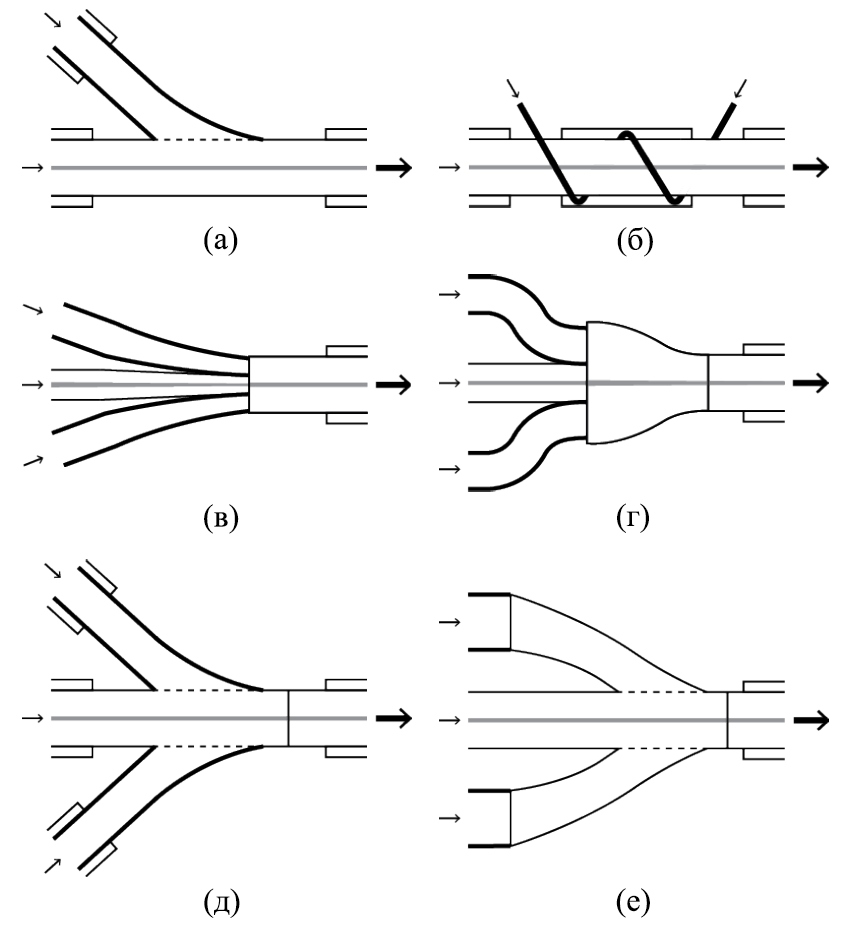
\includegraphics [scale=0.4] {taper_review_3_3}
  \caption{Подходы при реализации объединителей из волокон с полимерной оболочкой: (a) боковая накачка, (б) распределенная боковая накачка, (в) жгут тейпированных волокон, (г) сплавленный волоконный жгут с тейпированным промежуточным волокном, (д) MM волокна, приваренные к сигнальному волокну, (е) MM волокна, приваренные к сигнальному волокну через схлопнутую капиллярную трубку.}
  \label{img:taper_review_3_3}
\end{figure}

\item{\textit{Распределенная боковая накачка}. Подобна боковой накачке, описанной выше, за исключением того, что ММ волокно приварено к длинному участку активного волокна. Это позволяет производить накачку активного волокна с обеих сторон [23, 24].}

\item{\textit{Тейпированный волоконный жгут}. Несколько волокон накачки плавятся вместе, тейпируются и привариваются к активному волокну. Такой жгут может иметь
сигнальное волокно в центре конструкции [25-29].}

\item{\textit{Сплавленный волоконный жгут с тейпированным промежуточным волокном}. К сплавленному волоконному жгуту приварено промежуточное волокно. Это промежуточное волокно тейпировано и приварено к активному волокну с двойной оболочкой [30].}

\item{\textit{MM волокна, приваренные к сигнальному волокно}. Несколько тейпированных MM волокон сплавляются с SM волокном и привариваются к волокну с двойной оболочкой [31, 32].}

\item{\textit{MM волокна приварены к сигнальное волокно через схлопнутую капиллярную трубку}. Несколько MM волокон монтируются в капиллярной кварцевой трубке. Затем эта трубка тейпируется, схлапывается и приваривается к волокну. Сигнальное волокно с приваренной капиллярной трубкой приваривается к волокну с двойной оболочкой [33-35].}
\end{itemize}

Технология объединения с помощью жгута тейпированных волокон была запатентована в 2004 [70]. На рис.~\ref{img:taper_review_3_4}(a) проиллюстрирован данный подход.

\begin{figure} [ht]
  \center
  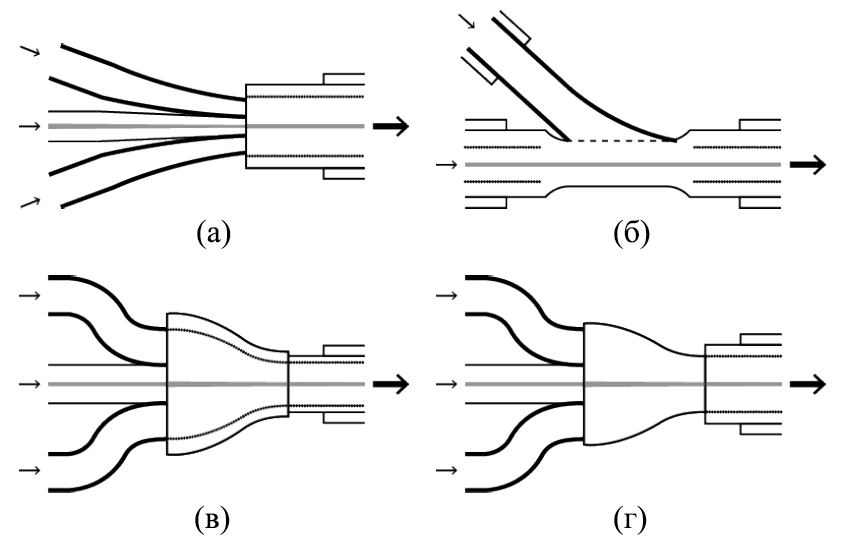
\includegraphics [scale=0.4] {taper_review_3_4}
  \caption{Подходы для создания объединителей из оптоволокна с воздушной оболочкой: (a) жгут тейпированных волокон, (б) боковая накачка, (в) сплавленный волоконный жгут с тейпированным промежуточным волокном и (г) сплавленный волоконный жгут со стравленным промежуточным волокном.}
  \label{img:taper_review_3_4}
\end{figure}

Недавно, для волокон с воздушной оболочкой был продемонстрирован новый перспективный подход, показанный на рис.~\ref{img:taper_review_3_4}(d). Несколько MM волокон сплавятся вместе с сигнальным волокном в волоконный жгут. Этот жгут приваривается к промежуточному волокну. Это волокно представляет собой кварцевое волокно без покрытия с сердцевиной со ступенчатым профилем ПП. Наружный диаметр промежуточного волокна уменьшается путем химического травления и приваривается к оптоволокну с воздушной оболочкой [75]. Излучение накачки удерживается воздушным промежутком (интерфейсом), а это означает, что наружный диаметр промежуточного волокна на тейпированном конце должен быть согласованным с внутренним диаметром воздушной оболочки PCF. Сигнал удерживается сигнальной сердцевиной, на которую не оказывает влияние процесс стравливания и тейпирования. Поэтому, данный подход потенциально может способствовать созданию объединителей с низким оптическими потерями.

Отметим, что мощность на выходе одномодовых или маломодовых волоконных лазеров за последние годы значительно увеличилась, и на данный момент составляет десятки кВт [82, 89-93]. Когерентное или некогерентное объединение излучения волоконных лазеров позволяет выполнять дальнейшее масштабирование выходной мощности. Когерентный объединение излучения одночастотных лазеров требует контроля фазы каждого источника. Это необходимо, чтобы гарантировать устойчивую интерференцию комбинированного пучка излучения. С другой стороны, некогерентное объединение не требует регулировки фазы. Это позволяет сделать более простую систему, но и менее спектрально чистое комбинированное излучение [94]. Установки для некогерентного спектрального объединения в свободном пространстве показали большой потенциал и позволили получить до 2 кВт выходной мощности с излучением близким к дифракционному пределу [95, 96]. В цельноволоконном подходе объединения излучения нет необходимости в объемных оптических компонентах, что позволяет получить жесткую и устойчивую лазерную систему. Недавно, жгуты тейпированных волокон показали высокий потенциал для реализации цельноволоконных компонентов для некогерентного объединения излучения [97]. Другим перспективным подходом является стравливание входных волокон и дальнейшее сплавление их вместе в капилляре из кварца с низким ПП [98]. С помощью данного подхода удалось объединить в общей сложности 4 кВт лазерного излучения [81].

%% ----------- наши результаты №1 [начало] ----------------------------

\subsubsection{Методика сварки объединителей}

\begin{enumerate}
  \item Вытягиваем промежуточный капилляр для создания «воронки».

\begin{figure} [ht]
  \center
  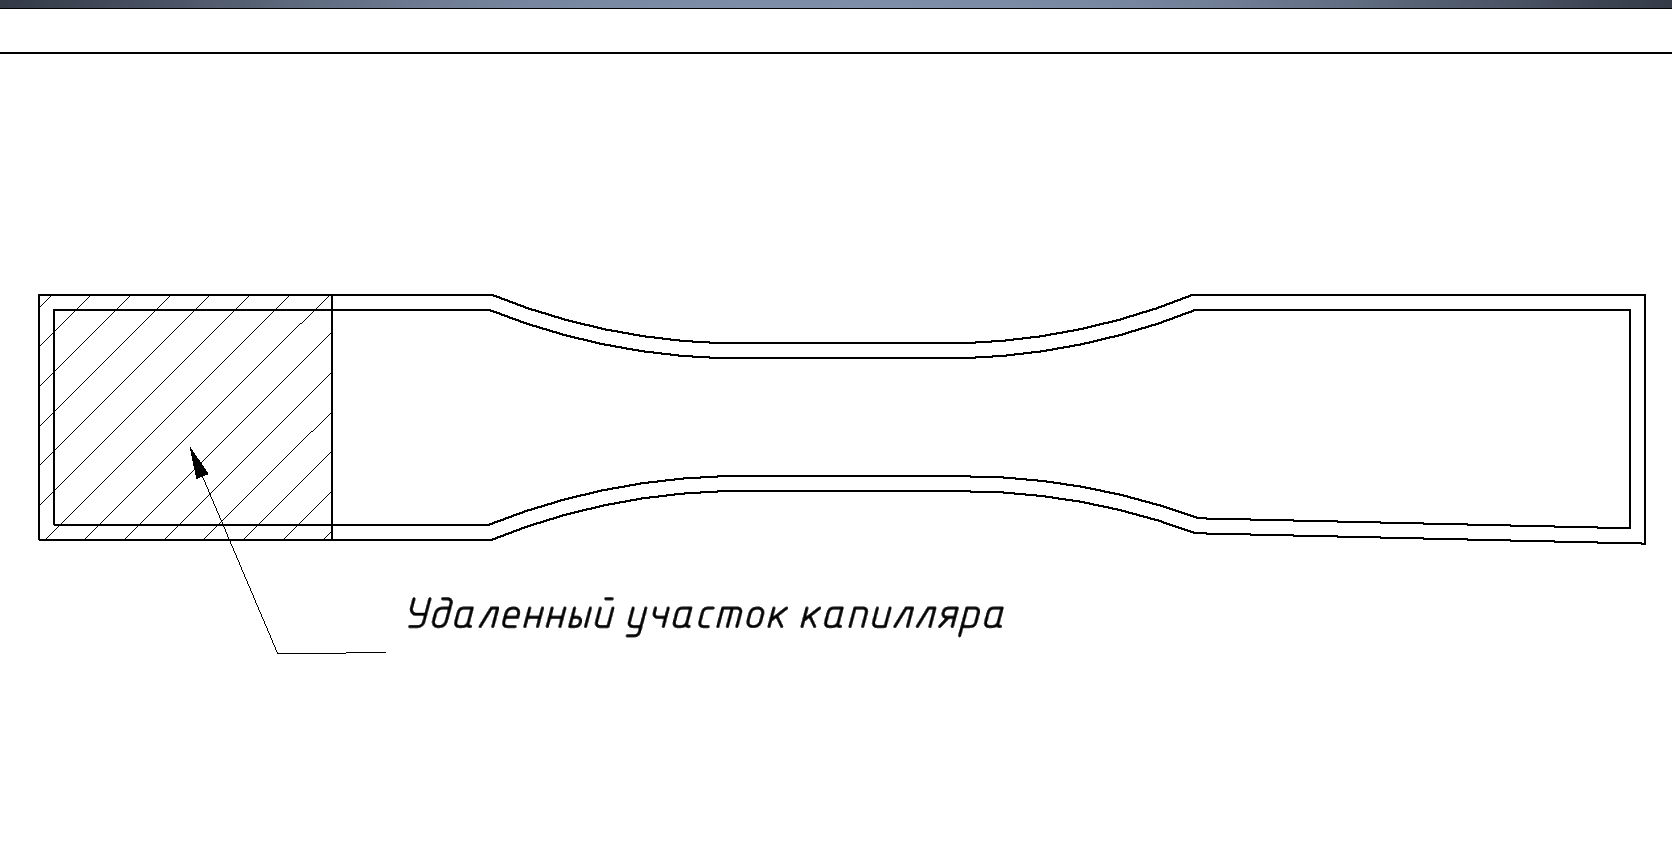
\includegraphics [scale=0.2] {comb_proc_1.png}
  \caption{Схема формирования заготовки из капилляра.}
  \label{img:comb_proc_1}
\end{figure}

  \item Монтируем в <<воронку>> зачищенные волокна накачки и закрепляем их УФ-отверждаемым клеем на торце капилляра.

\begin{figure} [ht]
  \center
  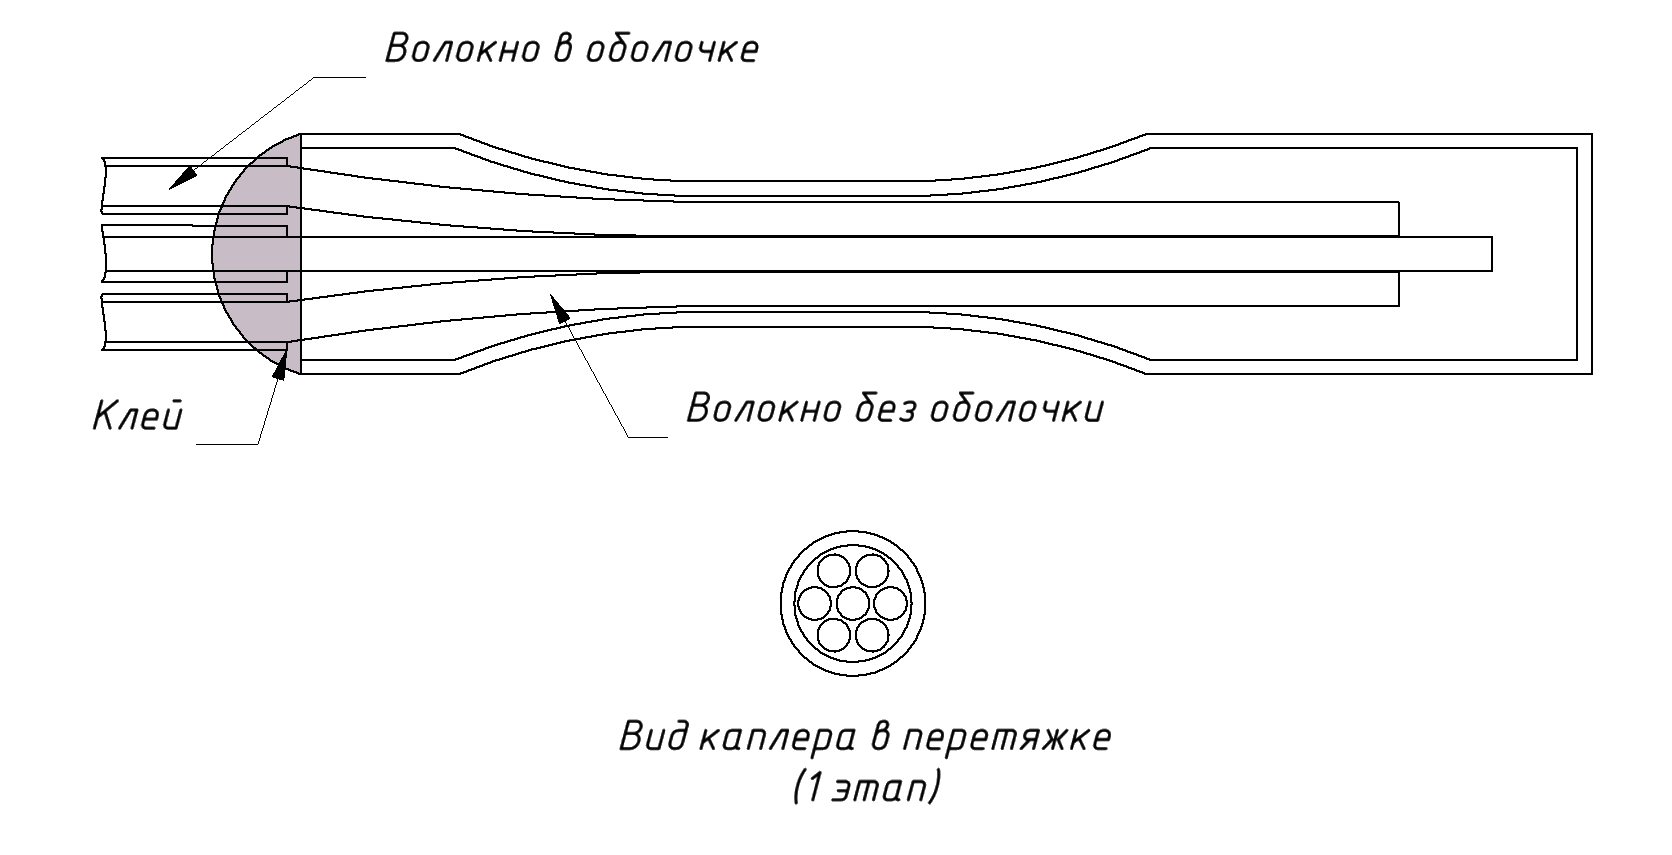
\includegraphics [scale=0.2] {comb_proc_2.png}
  \caption{Схема монтажа волокон в капилляре.}
  \label{img:comb_proc_2}
\end{figure}

  \item Производим повторную вытяжку и скалываем капилляр со жгутом волокон в месте минимальной перетяжки.
  \item Привариваем выходное волокно.
  \item Заливаем место сварки отражающим полимером СИЭЛ 305.
  \item Измеряем величину потерь излучения накачки на объединителе.
\end{enumerate}

Для оценки каждой составляющей потерь при создании объединителя были проведены предварительные детальные оценки потерь при тейпировании волокна. Для всех выполненных измерений использовалось импортное волокно 105/125 (NA=0,22).

\begin{figure} [ht]
  \center
  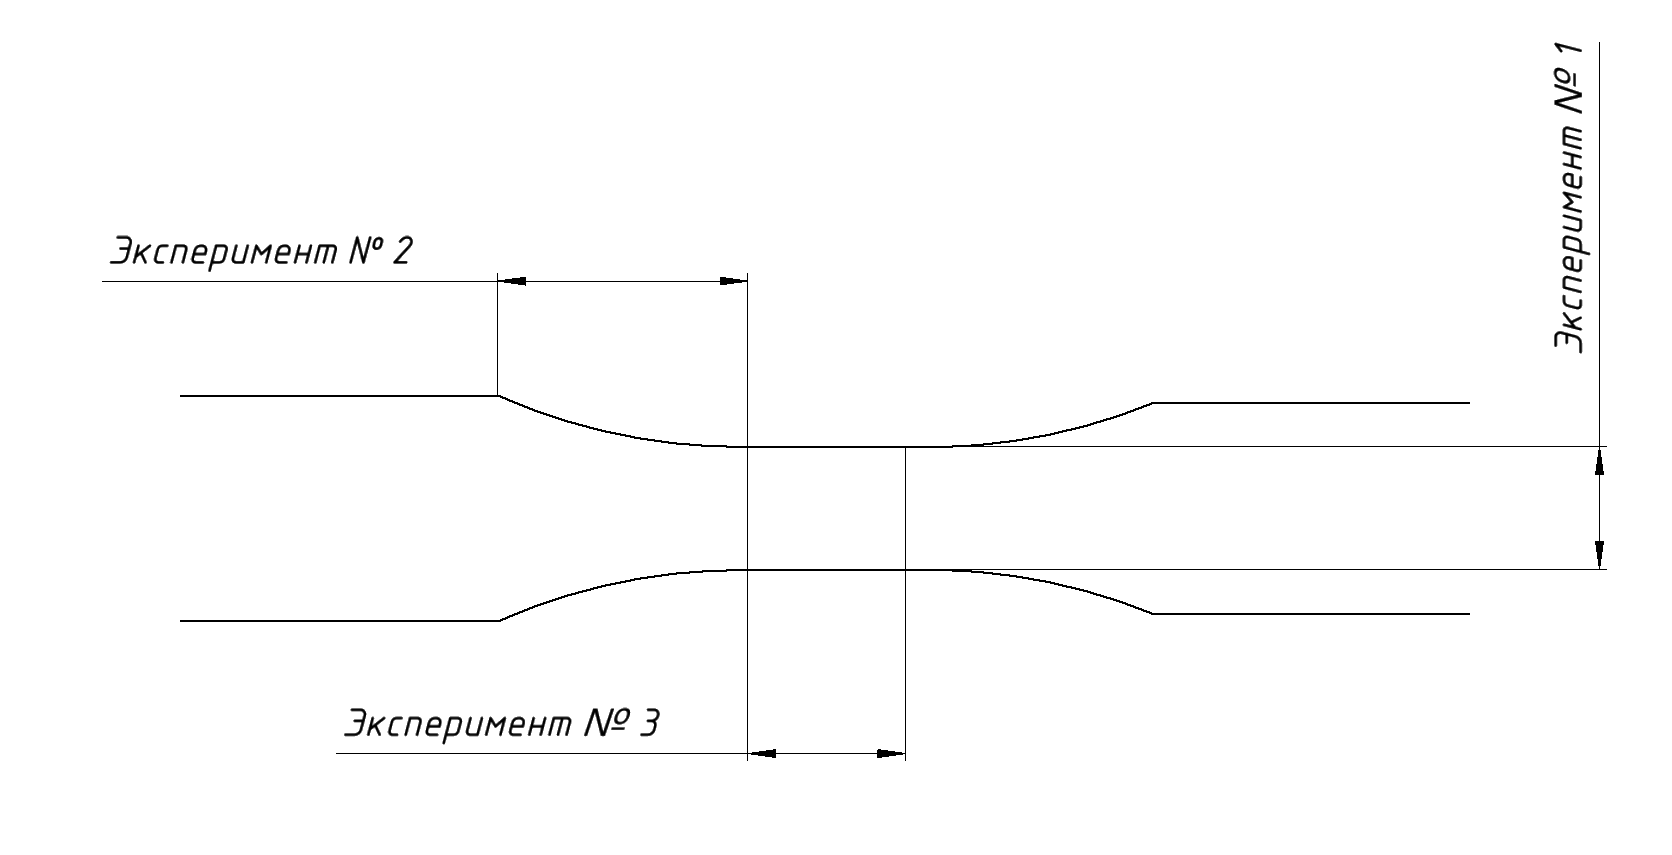
\includegraphics [scale=0.2] {comb_proc_3.png}
  \caption{Иллюстрация трех варьируемых параметров при оценке вносимых потерь: эксперимент №1 – диаметр перетяжки, эксперимент №2 – длина тейпера, эксперимент №3 – длина перетяжки.}
  \label{img:comb_proc_3}
\end{figure}

В первую очередь были измерены потери при варьировании диаметром перетяжки. Результаты экспериментов приведены на рис. 1.

\begin{figure} [ht]
  \center
  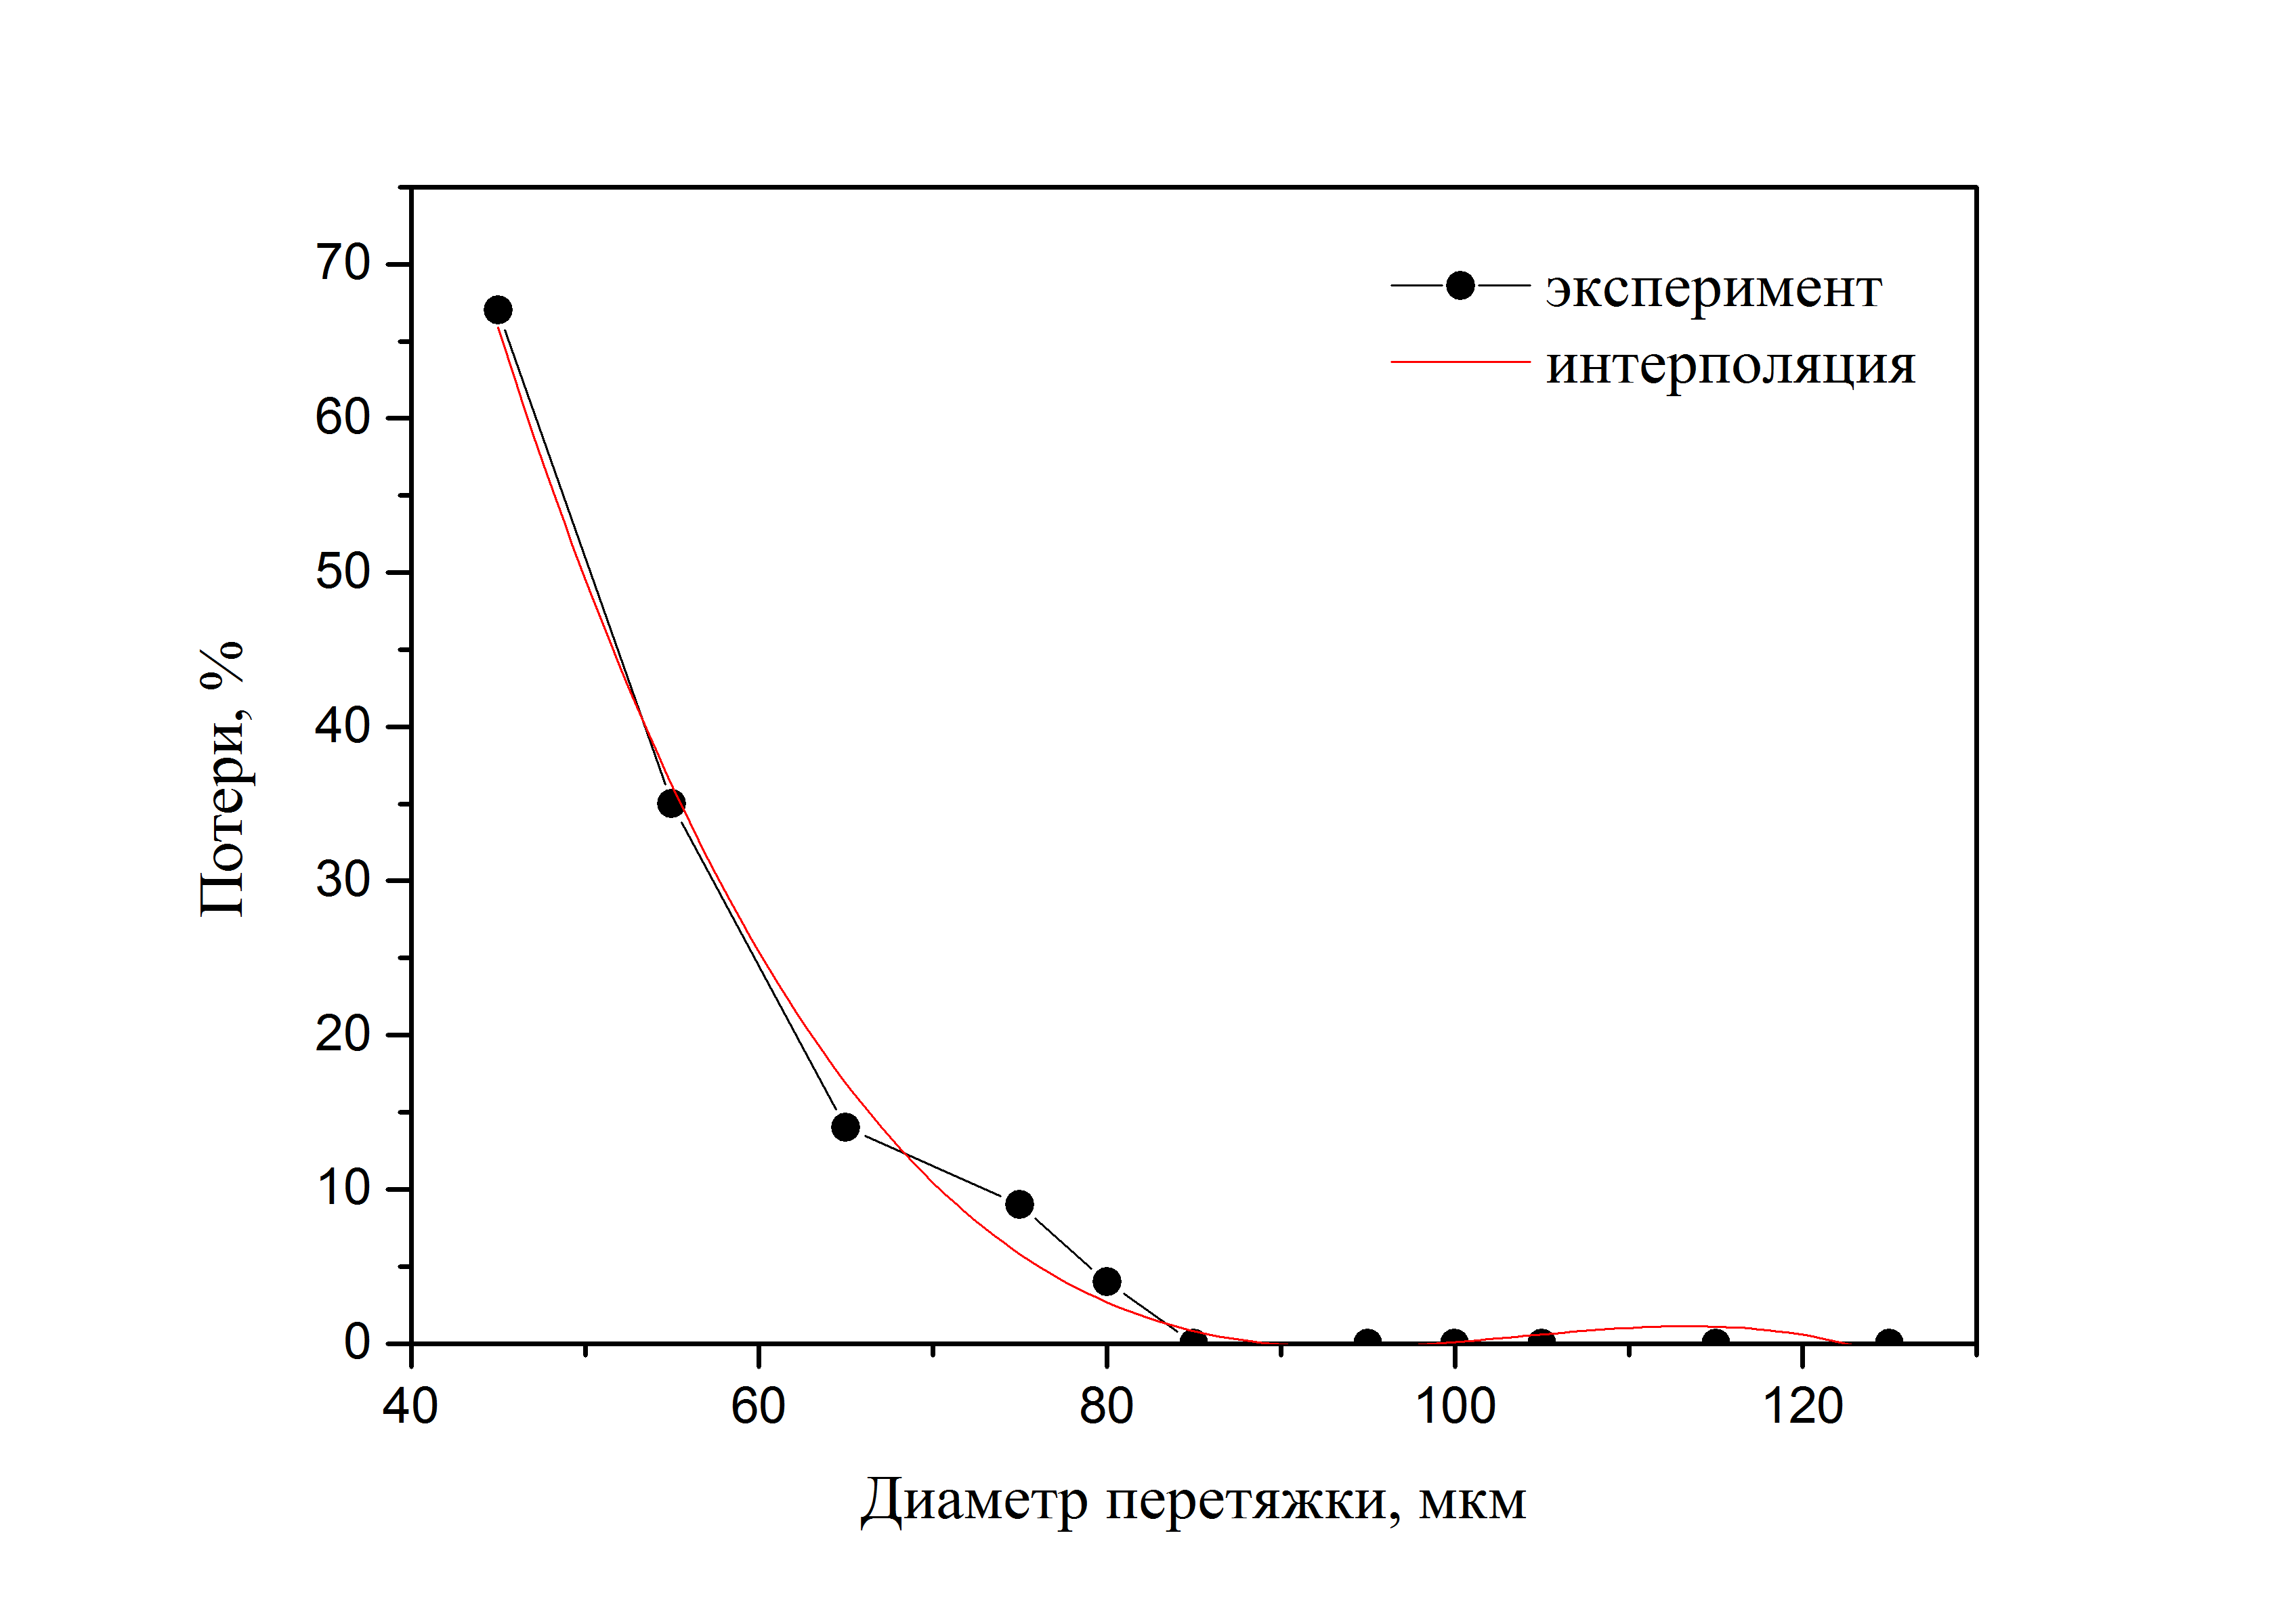
\includegraphics [scale=0.2] {comb_proc_4.png}
  \caption{График потери излучения при тейпировании волокна.}
  \label{img:comb_proc_4}
\end{figure}

Видно, что до перетяжки в 85 мкм (по оболочке) потерь на тейпировании не обнаружено. Следует отметить, что скалывание тейпера с диаметром перетяжки отличным от стандартного диаметра в 125 мкм представляет собой крайне трудоемкую задачу из-за многократного повторения процесса вытяжки и скалывания различными способами и установками (Vitran, Fujikure, ручной скалыватель – «ручка»). В среднем удачным получается каждое 3-5 скалывание.

Далее были измерены потери при изменении длины тейпера. Для исследования был выбран минимальный диаметр перетяжки без потерь из предыдущих измерений в 85 мкм. Длина вытягиваемого участка изменялась от 5 мкм до 50 мкм (предельное значение для установки Vitran) с шагом 5 мкм. При всех значениях потери не превысили 5~\% и в большей степени связаны с неидеальным сколом.

Также выполнены измерения потерь при варьировании длиной перетяжки. Величина изменялась в пределах от 5 мкм до 30 мкм с шагом в 5 мкм. Все оценки показали, что изменение длины перетяжки не вносит потерь в пропускание тейпера.

После второй вытяжки на установке Vitran GPX 3000 выполнено измерение диаметра перетяжки (внешний диаметр) для ввода корректного значения диаметра волокна в скалывателе Vitran LDC-400. Следует отметить, что произвести скалывание составного волокна (жгута) большого диаметра (с пустотами в структуре) удовлетворительного качества получается в одном из примерно 5 случаев. С учетом предварительной работы получение заготовок на данном этапе крайне трудоемки и продолжительный процесс.

\begin{figure} [ht]
  \center
  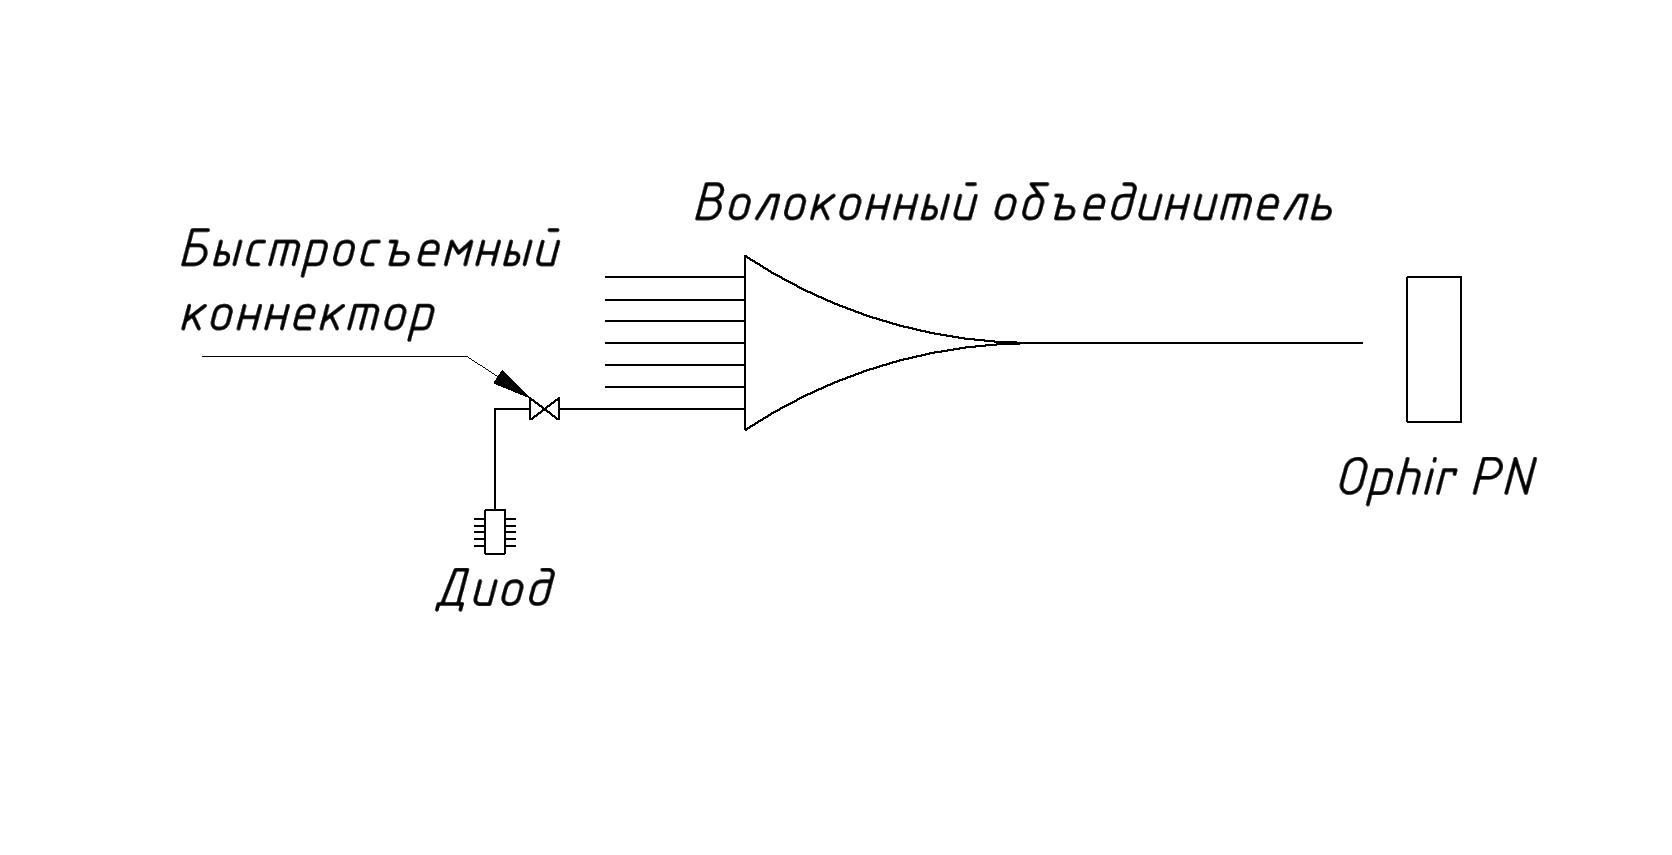
\includegraphics [scale=0.2] {comb_proc_5.png}
  \caption{Схема эксперимента по измерению потерь.}
  \label{img:comb_proc_5}
\end{figure}

\begin{figure} [ht]
  \center
  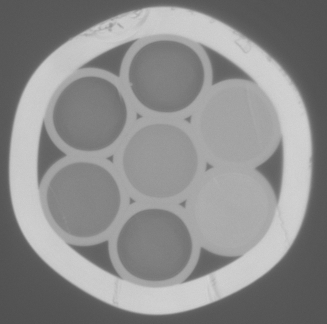
\includegraphics [scale=0.4] {comb_proc_6.png}
  \caption{Вид торца вытянутого объединителя (без выходного волокна), сколотого в перетяжке, и вид скола сбоку. Внутренний диаметр капилляра со жгутом волокон составляет 200 мкм.}
  \label{img:comb_proc_6}
\end{figure}

В таблице приведены лучшие результаты измеренных потерь в объединителе на данном этапе. Видно, что потери излучения по центральному каналу объединителя отсутствуют.

\begin{table} [htbp]
  \centering
  \parbox{16cm}{\caption{Потери на объединителе после скалывания (без выходного волокна).}\label{tbl:comb_res_2}}
  \begin{tabular}{| p{3cm} | p{4cm} |}
  \hline
  \hline
  Номер канала & Потери сигнала [\%] \\
  \hline
  1 & 0 \\
  2 & 3  \\
  3 & 13  \\
  4 & 6  \\
  5 & 4  \\
  6 & 3  \\
  7 & 5  \\
  \hline
  \hline
  \end{tabular}
\end{table}

Следует отметить, что на момент проведения экспериментов в наличии было волокна 105/125 только с числовой апертурой 0,22. Это не позволяет достоверно оценить потери после приваривания выходного волокна имеющего также числовую апертуру 0,22 в объединителе в конфигурации 7:1 (нарушение закона сохранения яркости). Обзорное исследование показывает, что в данном случае входное волокно должно иметь запас по апертуре по сравнению с выходным волокном. В данной конфигурации коммерчески доступны объединители накачки с входными волокнами 105/125 (NA=0,15) и выходным волокном 200/220 (NA=0,22).

Для проведения измерений потерь на стыке с выходным волокном было взято волокно Nufern с двойной оболочкой с диаметром первой оболочки 400 мкм и числовой апертурой 0,46. Это волокно было приварено к торцу волоконного объединителя.

\begin{figure} [ht]
  \center
  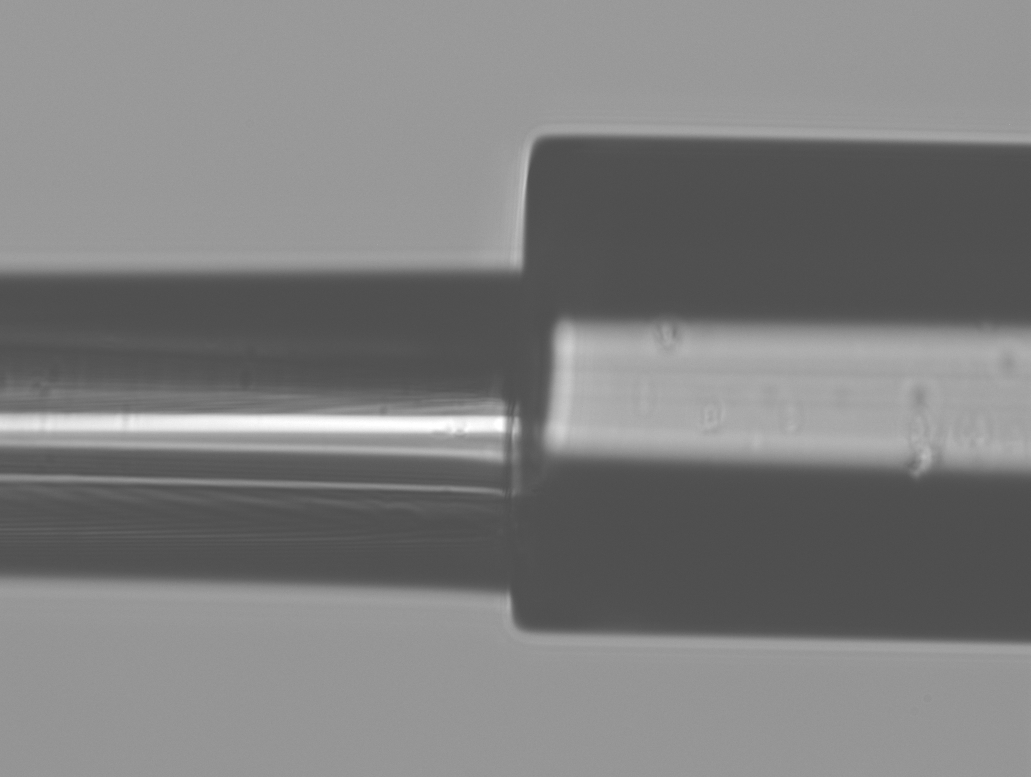
\includegraphics [scale=0.2] {comb_proc_7.png}
  \caption{Сварка объединителя (выход на 200 мкм) с выходным волокном с диаметром оболочки 400 мкм. Сварка выполнена на установке Vitran GPX 3000.}
  \label{img:comb_proc_7}
\end{figure}

В таблице ниже показаны значения измеренных потерь для нескольких каналов объединителя. После нанесения покрытия потери не превысили 14~\%, а минимальные потери по центральному каналу составили 5 %.

\begin{table} [htbp]
  \centering
  \parbox{16cm}{\caption{Потери на объединителе c приваренным выходным волокном (D=400~мкм).}\label{tbl:comb_res_2}}
  \begin{tabular}{| p{3cm} | p{4cm} |}
  \hline
  \hline
  Номер канала & Потери сигнала [\%] \\
  \hline
  1 & 8 \\
  2 & 14  \\
  3 & 8  \\
  4 & 7  \\
  5 & 8  \\
  6 & 6  \\
  \hline
  \hline
  \end{tabular}
\end{table}

Причина столь значительных потерь при вводе излучения с перетянутого объединителя в волокно со значительно большим диаметром (200 мкм слева против 400 мкм справа) и большой числовой апертурой (0,46 справа) пока однозначно не ясна. Можно предположить, что на торце объединителя мы имеем значительное увеличение апертуры при перетяжке (изначально 0,22), которое превышает величину 0,46. Для подтверждения (или опровержения) данного факта будут проведены измерения апертуры объединителя после перетяжки и до приваривания выходного волокна.

Таким образом, получено экспериментальное подтверждение возможности создания волоконных объединителей накачки на имеющемся в лаборатории 57-2 оборудовании. В конфигурации 7:1 с входными волокнами 105/125 (NA=0,22) и выходным волокном 20/400 (NA=0,46) достигнуты минимальные потери в 5~\% по центральному каналу. Следует отметить, что измерение потерь выполнялось при входной мощности порядка 350 мВт (длина волны 975 нм). Анализ литературы показывает, что при большей входной мощности потери могут уменьшаться (или в общем случае отличаются).

\textit{Проверка данного факта ппоказала, что ...}

Для получения пригодных к внедрению экспериментальных образцов необходима тонкая и кропотливая оптимизация параметров процесса вытяжки (как заготовки из капилляра, так и объединителя) и сварки.

Для уменьшения потерь излучения были изготовлены капилляры с отражающей оболочкой.

\textit{Получены следующие результаты}

Далее на объединителе с выходным волокном 200/220 (NA=0,22), в качестве входного использовано волокно 105/125 с числовой апертурой 0,15.

\textit{Получены следующие результаты}

%% ----------- наши результаты №1 [конец] ----------------------------

\subsection{Изготовление сплавленных объединителей накачки/сигнала}

На рис.~\ref{img:taper_review_6_5} показан объединитель и изображения трех его главных составляющих. Изображение поперечного сечения пассивного транспортного волокна с двойной оболочкой показано на рис.~\ref{img:taper_review_6_5}(b). Воздушная оболочка волокна видна как кольцо с близко расположенными отверстиями, окружающими центральную жилу оптоволокна. У волокна есть сигнальная сердцевина с MFD=15 мкм и диаметром оболочки накачки 133 мкм. Изображение поперечного сечения сплавленного волоконного жгута показано на рис.~\ref{img:taper_review_6_5}(d). Сигнальное волокно в центре окружено 7 волокнами накачки. Волокна накачки -- это волокна с NA=0,22 и диаметром сердцевины и оболочки 105 мкм и 125 мкм, соответственно. Сигнальное волокно –- это волокно со ступенчатым профилем ПП и отсечкой мод более высокого порядка при длина волны 980 нм, MFD=15 мкм, а диаметр оболочки 160 мкм. Изображение поперечного сечения тейпера показано на рис.~\ref{img:taper_review_6_5}(c). Функция тейпера заключается в воде излучения накачки из волокон накачки волоконного жгута в оболочку, при этом тейпер уменьшает площадь оболочки накачки. Это снижение увеличивает поглощение накачки в активном волокне.

\begin{figure} [ht]
  \center
  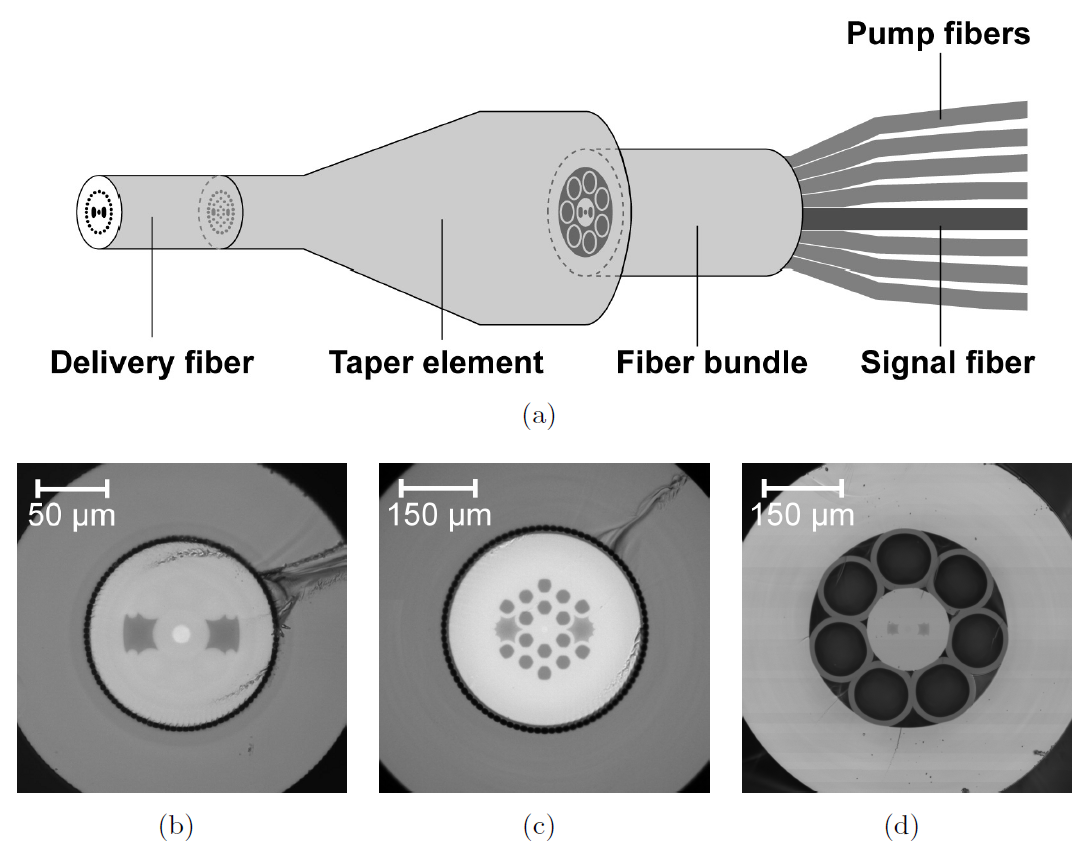
\includegraphics [scale=0.4] {taper_review_6_5}
  \caption{(a) Изображение сплавленных объединителя накачки/сигнала 7+1x1. (b) -- (d) изображения поперечного сечения (b) транспортного волокна, (c) тейпера и (d) волоконного жгута.}
  \label{img:taper_review_6_5}
\end{figure}

\begin{figure} [ht]
  \center
  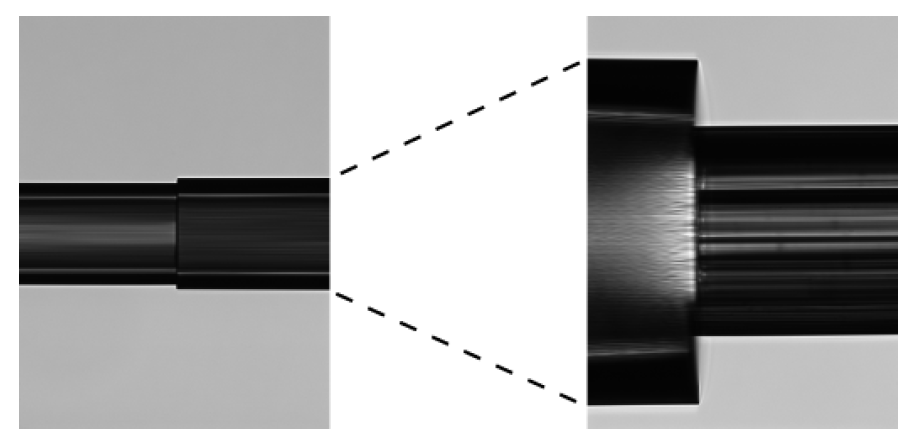
\includegraphics [scale=0.4] {taper_review_6_6}
  \caption{Изображения двух сварок в объединителе. Слева показана сварка между пассивным транспортным волокном и тейпированным концом тейпера. Справа показана сварка между тейпером и сплавленным волоконным жгутом. Пунктирная линия поясняет тейпирование элемента.}
  \label{img:taper_review_6_6}
\end{figure}

Одновременно элемент тейпера обеспечивает ввод сигнального излучения из сердцевины в сигнальное волокно волоконного жгута (при конфигурации с обратной или встречной накачкой). У тейпера есть воздушная оболочка с внутренним диаметром 400 мкм на нетейпированном конце. Когда тейпер приваривается к волоконному жгуту все волокна накачки находятся в пределах воздушной оболочки тейпера. На тейпированном конце диаметр воздушной оболочки равен 133 мкм и согласован с диаметром транспортного волокна. Соотношение между диаметром сердцевины накачки и NA излучения накачки в тейпированном многомодовом волокне определяется уравнением~\eqref{eq2.24}. Из него следует, что у транспортного волокна с максимальным NA=0,6 при тейпировании с коэффициентом 3, объединителем будет поддержано излучение накачки с NA < 0,20. Центр тейпера -- основанная на F-стержне структура с двойной сердцевиной. Минимальная длина тейпера, гарантирующая низкие потери как накачки, так и сигнала, определяется низким NA сигнального излучения, а не высоким NA излучения накачки. Поэтому используется 15-миллиметровый линейный тейпер. Волокно тейпера сужено с помощью установки для обработки стекла GPX от Vytran [58]. Путем контроля мощности нагревателя предотвращается схлопывание отверстий воздушной оболочки. Сплавление волоконного жгута и сварка также выполняются на установке GPX. Две сварки объединителя показаны на рис.~\ref{img:taper_review_6_6}. Сварка между транспортным волокном и тейпированным концом тейпера показана в левой части, а сварку между нетейпированным концом элемента тейпера и сплавленным жгутом показана справа. Для предотвращения схлопывания отверстий воздушной оболочки сварка выполняется при низкой температуре. Были измерены выходные характеристики объединителя как для каналов накачки, так и для сигнального канала. Потери при передачи накачки измерены с помощью коммерчески доступного одиночного диода на 915 нм с NA=0,15. Диод в свою очередь был приварен к каждому из 7 каналов. Средняя потеря мощности накачки составила 0,13 дБ, а максимальная потеря мощности -- 0,16~дБ. Сигнальные потери измерены с помощью источника поляризованного излучения с длиной волны 1060 нм. Источник был приварен к сигнальному волокну сплавленного волоконного жгута и измерены PER излучения на выходе и потери через объединитель. Потеря сигнала составила 0,52 дБ, а поляризационное соотношение PER=20 дБ.

Это даст самое большое значение для минимальной длины тейпера.

\noindent
\textbf{А1. Минимальная длина тейпера из одномодового волокна при линейном профиле тейпера}

Для линейного профиля тейпера наклон тейпера $dr/dz$ будет одинаковым по всей длине тейпера. Максимальная длина биений $L_{B,max}$ и полное соотношение тейпера ($TR$) поэтому определят длину адиабатического тейпера ($L$). Соотношение тейпера здесь определяется как $TR=r_1/r_2$, где $r_1$ и $r_2$ -- радиус сердцевины волокна на нетейпированном и тейпированном концах, соответственно. Уравнение \eqref{eq2.16} можно привести к
\begin{equation}\label{eqA1}
  \frac{dr}{dz}\le\frac{r}{L_B},
\end{equation}
\begin{equation}\label{eqA2}
  \frac{r_1-r_2}{L}\le\frac{r_2}{L_B},
\end{equation}
\begin{equation}\label{eqA3}
  L\ge L_B\frac{r_1-r_2}{r_2},
\end{equation}
\begin{equation}\label{eqA4}
  L\ge(TR-1)L_{B,max}.
\end{equation}
В правой части уравнений выше $r$ аппроксимирован $r_2$. Это даст самое большое значение для минимальной длины тейпера.

\noindent
\textbf{А2. Минимальная длина тейпера из многомодового оптоволокна при линейном профиле тейпера}

Для линейного профиля тейпера наклон тейпера $dr/dz$ будет одинаковым по всей длине тейпера. Радиус сердцевины волокна на нетейпированном и тейпированном концах -- $r_1$ и $r_2$, соответственно. Соответствующий диаметр сердцевины оптоволокна -- $D_1$ и $D_2$. Уравнение \eqref{eq2.20} можно привести к
\begin{equation}\label{eqA5}
  \frac{dr}{dz}\le\frac{\tg\theta_z}{2},
\end{equation}
\begin{equation}\label{eqA6}
  \frac{r_1-r_2}{L}\le\frac{\tg\theta_z}{2},
\end{equation}
\begin{equation}\label{eqA7}
  L\ge\frac{2(r_1-r_2)}{\tg\theta_z},
\end{equation}
\begin{equation}\label{eqA8}
  L\ge\frac{D_1-D_2}{\tg\theta_z}.
\end{equation}


\subsection{Стенд выходного контроля параметов изготовленных объединителей накачки}

Для получения прав на применение необходимо, чтобы пассивные оптические разветвители соответствовали некоторым международным стандартам, установленным Telcordia Technologies (ранее Bellcore). Также для обеспечения обратной связи в процессе изготовления важна достаточная характеристика сборных ответвителей. Сверхнормативная потеря и спектральное распределение света в ответвителе являются двумя основными особенностями, которые решают качество расположенного в ответвителе устройства [33].

%\subsection{Параметры каплеров}

Производительность каплеров количественно оценивается жерез ряд характеристик [11]. Наиболее важные характеристики любого каплера -- это коэффициент разделения (splitting ratio) и избыточные потери (excess loss).

\subsubsection*{\textbf{Коэффициент разделения (Coupling Ratio, CR)}}

Коэффициент разделения или коэффициент связи есть мера распределения мощности в выходных оптоволоконных каналах при заданной длине волны. Коэффициент разделения определяется, как соотношение мощностей, измеренных в данных каналах [11, 36]. Коэффициент связи в связанном канале определяется, как

\begin{equation}\label{eq_ch3_2.28_2}
  CR=\frac{P_C}{P_T+P_C}\times 100\%.
\end{equation}
Аналогично, коэффициент связи в проходном канале (throughput port) определяется как
\begin{equation}\label{eq_ch3_2.29}
  CR=\frac{P_T}{P_T+P_C}\times 100\%.
\end{equation}
Коэффициент разделения описывает то, как излучение на входе каплера распределяется между выходными каналами. CR может варьироваться от 0 до 100~\%. Он всегда рассчитывается для определенной длины волны. Последнее имеет место в силу наличия зависимости коэффициента связи от длины волны.

\subsubsection*{\textbf{Избыточные потери (Excess Loss, EL)}}

Избыточные потери в каплере -- это доли входной мощности, которая не дошла до выходных каналов. Обычно она выражается в дБ. Для входной мощности $P_I$ и выходной $P_C$ и $P_T$ в связанном и проходном каналах соответственно, избыточные потери выражаются как
\begin{equation}\label{eq_ch3_2.30}
  EL=-10\log\left(\frac{P_T+P_C}{P_I}\right).
\end{equation}
Для устройства с $n$ выходными каналами,
\begin{equation}\label{eq_ch3_2.31}
  EL=-10\log\left(\sum_{j=1}^n \frac{P_j}{P_I}\right).
\end{equation}
Важным показателем является общая эффективность каплера. Она отвечает за потери энергии вследствие рассеяния [37]. Избыточные потери в каплере хорошего качества обычно составляют менее 0,1 дБ.

\subsubsection*{\textbf{Вносимые потери (Insertion Loss, IL)}}

Вносимые потери -- это суммарная потеря пропускаемой мощности при прохождения через каплер по тому или иному пути (каналу). Они определяются соотношением доступной (на входе) мощности в данном выходном канале к исходной мощности [11, 36]:
\begin{equation}\label{eq_ch3_2.32}
  IL=-10\log\frac{P_C}{P_I}.
\end{equation}
Вносимые потери являются суммой избыточных потерь и коэффициента связи (выраженного в дБ) вдоль пути прохождения излучения. Таким образом, вносимые потери 3 дБ-го каплера составляют более 3 дБ. Вносимые потери является основным параметром для проектировщиков оптоволоконных систем. Значение используется при вычислении баланса мощности (power budget in link designs).

\subsubsection*{\textbf{Направленность (Directivity, DIR)}}

Направленность каплера -- это мера отражённой мощности. Она показывает, насколько хорошо каплер передаёт излучение в выходные каналы, и количественно оценивает величину отраженного излучения внутри устройства. Выражаемая в дБ, она определяется, как отношение мощности, возвращённой входному каналу, к введённой входной мощности [11, 36, 38].
\begin{equation}\label{eq_ch3_2.33}
  DIR=-10\log\frac{P_R}{P_I}
\end{equation}
Фактически, на практике для измерения направленности все выходные каналы погружаются в жидкость с согласованным показателем преломления (иммерсионная жидкость). Эта процедура гарантирует, что отражения Френеля (из-за разницы показателей преломления на границе между оптоволокном и воздухом) не дает вклад в измеряемую отражённую мощность. Направленность в зарубежной литературе иногда называют изоляцией передающего конца (nearend-isolation).

%\subsection{Измерение характеристик каплера}

Измерение характеристик каплеров важно для подтверждения и количественной оценки производительности после его упаковки. Это необходимо в силу того, что во время упаковки клей (оптический цемент), который используется для крепления каплера к кварцевой подложке, часто в процессе отверждения дает небольшое натяжение. Это в свою очередь приводит к небольшому изменению оптических характеристических, таких как коэффициент разделения и отклик по длинам волн.

Коэффициент разделения и вносимые потери измеряются как во время, так и после изготовления [39]. В дополнение к измерению потерь EL, IL, коэффициенту CR и направленности DIR, измерение характеристик включает в себя измерение отклика по длинам волн (wavelength response) для всех типов каплеров и изоляцию длины волны (wavelength isolation) для WDM компонентов. На рис.~\ref{img:taper_review_ch3_2_8} изображена схема измерения коэффициента связи, вносимых потерь IL и потерь, зависящих от поляризации. Излучение нескольких источников подсоединяется к каплеру Nx1, который в свою очередь подсоединяется к контроллеру поляризации. В такой конфигурации можно проводить измерения с использованием ряда длин волн, равномерно расположенных в требуемом спектральном диапазоне. Выходной сигнал контроллера поляризации соединяется с испытуемым каплером. Выходные концы каплера подсоединяются к двухканальному фотодетектору, используя оптоволоконные адаптеры. Детекторы InGaAs в свою очередь подключаются к ПК через карту сбора данных (DAC card).

\begin{figure} [ht]
  \center
  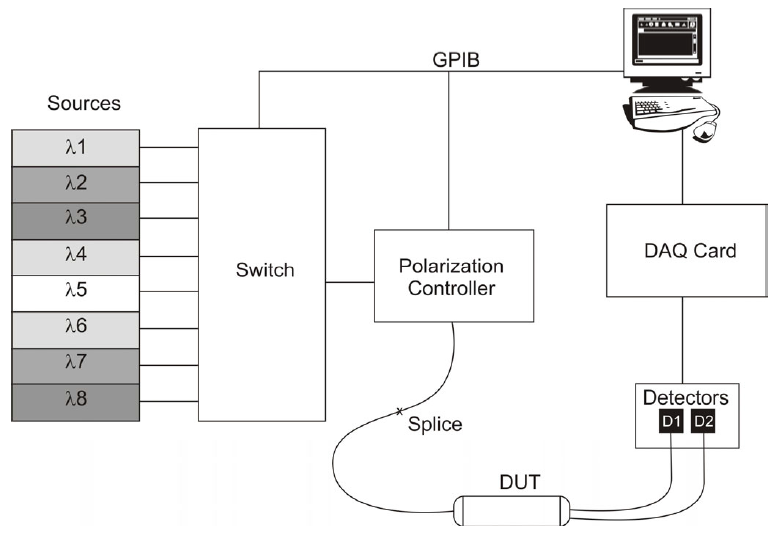
\includegraphics [scale=0.4] {taper_review_ch3_2_8}
  \caption{Схема измерения показателей каплера с использованием нескольких лазерных источников.}
  \label{img:taper_review_ch3_2_8}
\end{figure}

Что касается измерения отклика каплера на длины волн, то излучение от широкополосного источника подается на входное оптоволокно, а выход подсоединяется к оптическому спектральному анализатору (OSA). Используемые широкополосные источники белого света являются либо вольфрам-галогенновой лампой, либо светодиодным источником. Данные измерений также могут быть использованы для оценки спектрального отклика устройства с использованием метода аппроксимации (curve fitting method). Для измерения выхода мощности из направленного порта, которое обычно осуществляется в конце цикла измерения, порты двух выходов погружаются в жидкость согласования показателей преломления для того, чтобы избежать измеренной мощности от отражений Френеля. Обратные оптические потери измеряются с помощью измерителя обратного отражения. В этом устройствах излучение вводится в оптоволокно и следует назад к фотодетекторам с помощью оптических циркуляторов. Температурозависимые потери (Temperature Dependent Loss, TDL) является другим важным параметром, который показывает изменение вносимых потерь каплера, когда его температура колеблется между максимальным и минимальным значением рабочих температур. Типичная величина температурозависимых потерь составляет 0,2~дБ.

\newpage
\section{Cигнальные объединители излучения волоконных лазеров киловаттного уровня}

Цельноволоконные сигнальные объединители для некогерентного объединения лазерного излучения -- это ключевой компонент для стабильного получения нескольких кВт выходной лазерной мощности. Объединитель соединяет 7 волоконных лазеров в одномодовое или многомодовое волокно. У входных сигнальных волокон диаметр сердцевины равен 17 мкм, и у выходного ММ волокна диаметр сердцевины –- 100 мкм. В тейпированной области излучение постепенно выходит из сердцевины волокна и захватывается фторовой оболочкой обсадного капиляра. Объединитель протестирован до суммарной выходной мощности в 2,5 кВт.

\subsection{Изготовление сигнальных объединителей}

В работе [58] дано описание технологии создания сигнальных объединителей.
Для изготовления использована установка для обработки стекла GPX от Vytran [58]. Она используется для сплавления жгутов, сужения (тейпирования) и сваривания. На рис.~\ref{img:taper_review_5_1} показан вид объединителя. Сигнальные волокна представляют собой одиночные оптические волокна со ступенчатым профилем ПП, диаметром сердцевины 17 мкм и диаметром оболочки 125 мкм. Жгут из 7 волокон вставлен в легированную фтором кварцевую капиллярную трубку. Эти волокна в капиллярной трубке сплавляются и тейпируются до образования монолитной структуры. Тейпированный элемент будет действовать как ММ волновод с сердцевиной, состоящей из сплавленных волокон и оболочки, сформированной капиллярной трубкой с низким ПП. На рис.~\ref{img:taper_review_5_1}(b)-(c) показано поперечное сечение вдоль сплавленного и тейпированного жгута. Жгут тейпированных волокон приварен к ММ волокну с диаметром сердцевины 100 мкм и диаметром оболочки 660 мкм и числовой апертуры 0,22. Чтобы увеличить механическую прочность соединения, внешний диаметр ММ волокна уменьшен путем химического травления кварцевой оболочки. На рис.~\ref{img:taper_review_5_1}(d) показан профиль стравленного ММ волокна. На рис.~\ref{img:taper_review_5_1}(e) дано изображение сварного соединения.

\begin{figure} [ht]
  \center
  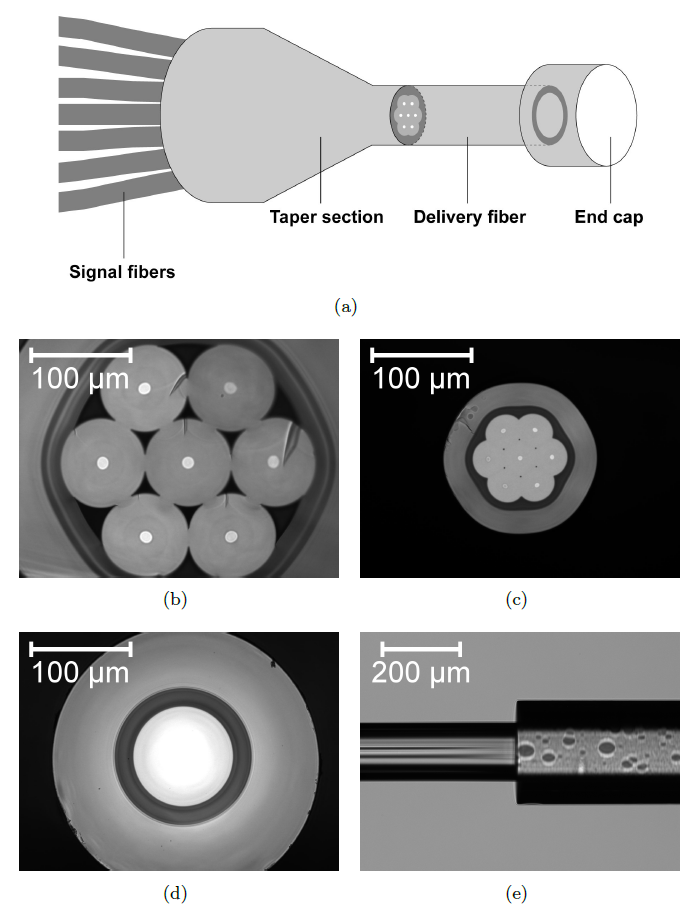
\includegraphics [scale=0.4] {taper_review_5_1}
  \caption{(a) Схематическая иллюстрация сигнального объединителя. (b)-(c) Изображения профиля тейпера. Диаметр 7 волокон составляет 255 мкм и 95 мкм, соответственно. (d) Изображение торца многомодового оптоволокна. На изображении показано стравленное волокно для улучшения согласования диаметра сплавленного жгута. Диаметр сердцевины равен 100 мкм. (e) Изображение жгута тейпированных волокон (справа), приваренного к стравленному ММ волокну.}
  \label{img:taper_review_5_1}
\end{figure}

Чтобы избежать обратного отражения в сигнальном объединителе, ММ волокно оснащается мощным разъемом от компании Optoskand [113]. Этот разъем состоит из алюминиевого держателя, в котором установлено ММ волокно. В нем также смонтирован 20 мм кварцевый наконечник (end cap), приваренный к волокну. Выходная поверхность наконечника имеет антиотражающее покрытие, которое снижает потери в разъеме. Разъем сконструирован так, чтобы противостоять очень высоким уровням обратного отражения от обрабатываемой детали, которое имеет место при обработке материалов. Разъем рассчитан на работу при 5 кВт средней мощности с потерями менее 3~\%. На рис.~\ref{img:taper_review_5_2}(a) показан вид разъема. Чтобы достигнуть высокой эффективности с низкими потерями, крайне важно добиться сильной оптической связи между волокном и наконечником. На рис.~\ref{img:taper_review_5_2}(b) показана оптическая связь без дефекта между 100~мкм  волокном (наружный диаметр 660 мкм) и сплавленным кварцевым наконечником, если смотреть через 20-миллиметровый наконечник. И сердцевина ММ волокна, и наконечник -- чистый кварц.

\begin{figure} [ht]
  \center
  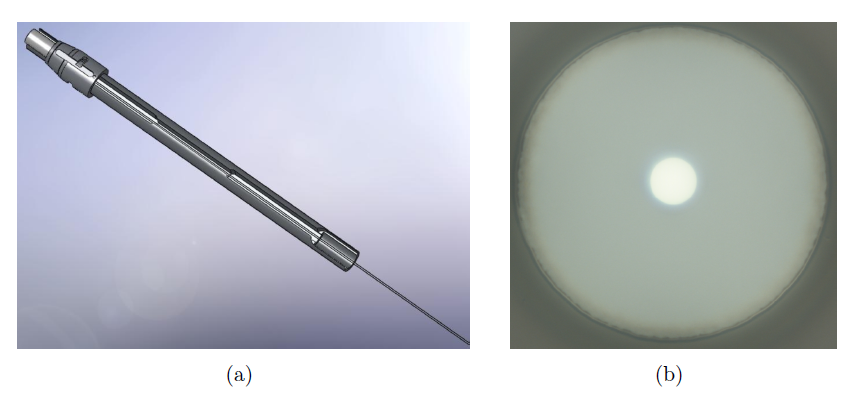
\includegraphics [scale=0.4] {taper_review_5_2}
  \caption{(a) Открытый QB разъем пигтейла от Optoskand. (b) Оптическая связь между волокном с сердцевиной 100 мкм и сплавленным кварцевым наконечником. Широкополосное излучение направлено в сердцевину ММ волокна. Это означает, что нет никакой границы показателя преломления, и оптическая связь осуществляется с минимальными потерями и минимальным обратным отражением.}
  \label{img:taper_review_5_2}
\end{figure}

\subsection{Стенд для испытания сигнальных объединителей}

Сначала объединитель испытывается на малой проходной мощности. Были измерены потери при передаче энергии, оптическое поле в дальней зоне и значения M$^2$ при объединении 7 сигнальных каналов. Все измерения выполнены с помощью волоконного лазера с выходной мощностью 1 Вт на длине волны 1060 нм. Для того, чтобы измерить потери при передаче энергии, волоконный лазер был приварен к каждому из сигнальных каналов объединителя. Потери для каждого из каналов приведены в табл.~\ref{tbl:5.1}. У всех каналов приблизительно одинаковый уровень потерь со средним значением 4,6~\%. При вводе излучения во все 7 каналов объединителя может быть измерено объединенное оптическое поле в дальней зоне, выходящее из ММ волокна. Это измерение выполнено при объединенной мощностьи на выходе в 1 Вт на длине волны 1060 нм. Измеренное заполнение NA соответствует 95~\% излучения, имеющего NA ниже 0,06. Используя профайлер Spiricon исследовано качество пучка излучения. Измеренное значение M$^2$ составило 6,8.

\begin{table} [htbp]
  \centering
  \parbox{15cm}{\caption{Потери сигнала в объединителе для каждого из 7 входных каналов.}\label{tbl:5.1}}
%  \begin{center}
  \begin{tabular}{| p{3cm} | p{4cm} |}
  \hline
  \hline
  Номер канала & Потеря сигнала [\%] \\
  \hline
  1 & 3,8 \\
  2 & 4,6  \\
  3 & 5,4  \\
  4 & 4,9  \\
  5 & 4,5  \\
  6 & 4,9  \\
  7 & 4,4  \\
  В среднем & 4,6  \\
  \hline
  \hline
  \end{tabular}
%  \end{center}
\end{table}

Для испытания объединителя на большой мощности использованы три непрерывных волоконных лазера мощностью 1 кВт (CW) производства Rofin-Sinar Laser GmbH [114]. Лазер имеет пассивное выходное волокно с диаметром сердцевины 20 мкм и дает одномодовое выходное излучение с BPP < 0,4 мм x мрад. Длина волны излучения составляет 1070 нм или 1080 нм. Волоконные лазеры киловаттного класса основаны на цельноволоконном генераторе. Оптическая эффективность составляет приблизительно 80~\% в зависимости от длины волны накачки. При этом можно достигнуть электрической эффективности до 38~\%.

Три кВт-ых волоконных лазера приварены к трем случайно выбранным каналам сигнального объединителя. Эти каналы имеют номера 4, 6 и 7, и, как оказалось, были центральным каналом и двумя боковыми каналами, разделенными одним волокном. Сварное соединение между транспортным волокном волоконного лазера и входным волокном объединителя сделано на сварочном аппарате Fujikura. Потери на сварке составили 4~\%. Мощность трех волоконных лазеров была установлена таким образом, чтобы мощность в каждом из входных каналов была приблизительно одинаковой. Объединенная мощность на выходе как функция входной мощности показана непрерывной линией на рис.~\ref{img:taper_review_5_3}.

\begin{figure} [ht]
  \center
  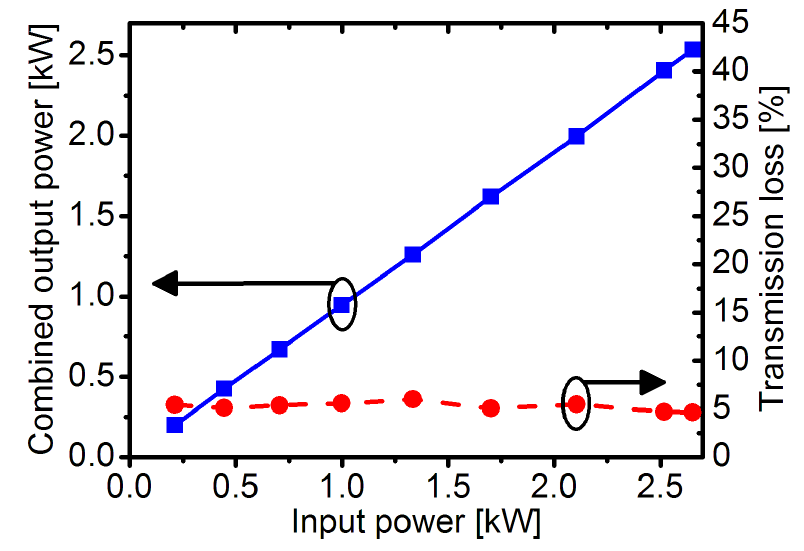
\includegraphics [scale=0.4] {taper_review_5_3}
  \caption{Суммарная мощность на выходе как функция входной мощности (непрерывная линия). Потери при передаче сигнального излучения в объединителе (пунктирной линия).}
  \label{img:taper_review_5_3}
\end{figure}

На рисунке пунктирной линией показаны потери при передачи сигнального излучения. Линейное поведение объединителя наблюдается без отклонений при больших мощностях и со средней потерей сигнала 5,3~\%. Наибольшая достигнутая мощность на выходе составляет 2,54 кВт. При данной величине мощности объединитель рассеивает 129 Вт сигнального излучения, при этом наблюдается незначительное увеличение температуры объединителя до 38 C$^\circ$. Это означает, что большая часть излучения успешно выведена оптически вместо того, чтобы быть поглощенной оболочкой. Качество пучка излучения исследовано с помощью монитора Primes Focus [115]. Измерение выполнялось при объединенной мощности в 600 Вт. Произведение 2.22 мм x мрад соответствует значению M$^2$=6,5. Эти значение находятся в превосходном согласии со значениями, измеренными при малой мощности. Распределение мощности в ближнем поле ММ волокна показано на рис.~\ref{img:taper_review_5_4}. На графике видно, что распространение не однородно. Наблюдается большой пик интенсивности в левой части. Вводом излучения во все каналы объединителя (вместо трех) можно добиться более равномерного распределения. Также считается, что распространение может быть сделано более однородным путем увеличения степени тейпирования волоконного жгута.

\begin{figure} [ht]
  \center
  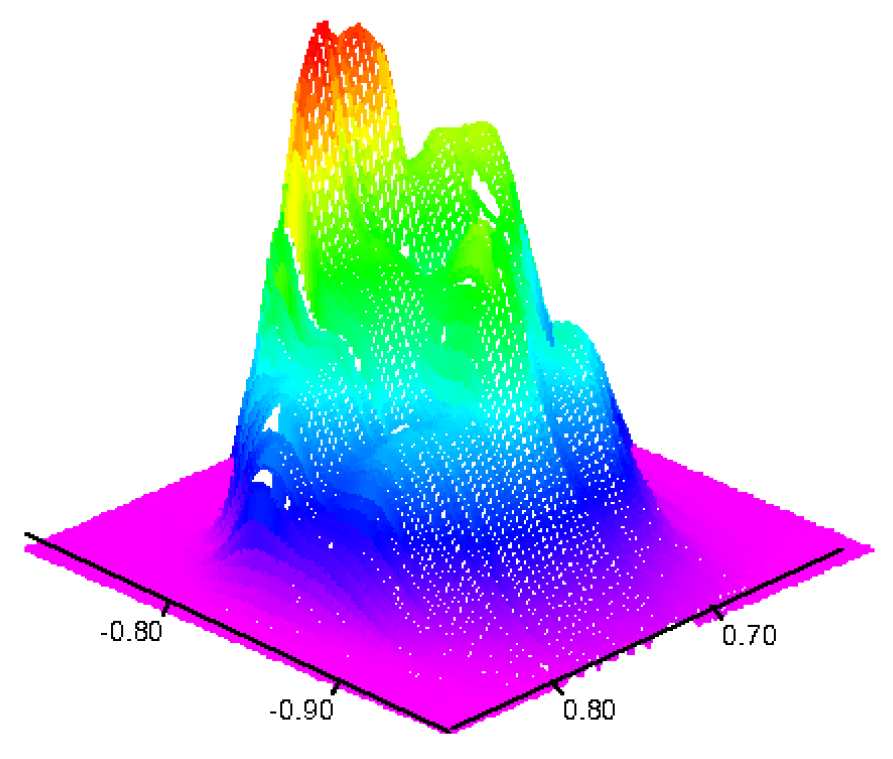
\includegraphics [scale=0.4] {taper_review_5_4}
  \caption{Распределение мощности в ближнем поле ММ волокна при объединенной мощности на выходе 600 Вт. Большее соотношение тейпера приведет к меньшему вкладу высокого ПП на тейпированном конце волоконного жгута. Это означает, что излучение будет менее ограничено этими вкладами и более «размажется» по всей ММ сердцевине.}
  \label{img:taper_review_5_4}
\end{figure}

\clearpage